\documentclass{article}
\usepackage[landscape]{geometry}
\usepackage{graphicx}
\usepackage{caption}
\usepackage{hyperref}
\usepackage{fancyhdr}

\captionsetup{font=Large}

\pagestyle{fancy}
\fancyhf{}
\rfoot{\href{https://www.wootenwealth.com}{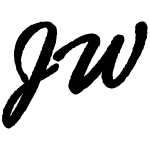
\includegraphics[width=1cm]{JW.png}}}
\fancyfoot[C]{Images or their data generally originated online.\\Find attributions in \href{https://www.ninetonoonsecrets.com}{the book} and \href{https://refs.ninetonoonsecrets.com}{its sources}.}
\setlength{\footskip}{32.05098pt}

\title{\vspace{-.5cm}\textit{Nine to Noon} - All Figures}
\author{\href{https://www.ninetonoonsecrets.com}{www.ninetonoonsecrets.com}}
\date{Wooten Wealth}


\begin{document}


\maketitle
\thispagestyle{empty}
\pagenumbering{roman} % Start Roman numbering

% [Content to be numbered in Roman]

\begin{figure}[!htb]
    \centering
    \fbox{\includegraphics[width=550pt]{pics-promo.png}}
\end{figure}

\pagebreak
\thispagestyle{empty}
\begin{center}
\Large{While waiting for your book, learn the fundamentals with a \href{https://www.stockmarketsecrets.exposed}{free course:}}
\end{center}
\begin{figure}[!htb]
    \centering
    \href{https://www.stockmarketsecrets.exposed}{{\includegraphics[width=450pt]{smse-promo.png}}}
\end{figure}
\pagebreak

\setcounter{page}{1}
\pagenumbering{arabic}

\begin{figure}[!htb]
    \centering
    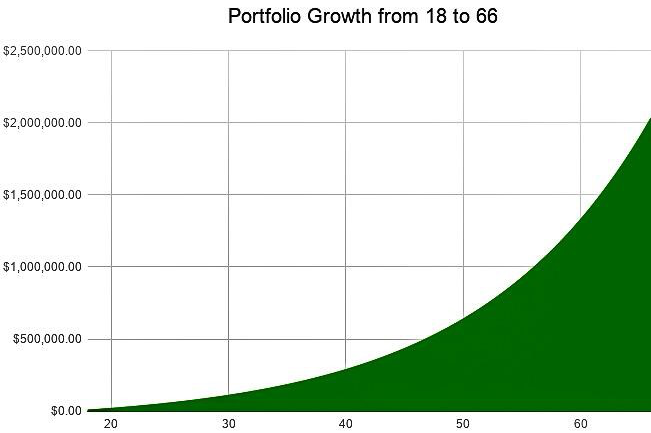
\includegraphics[width=\textwidth]{imgs/1.png}
    \caption{You're holding your savings and retirements right now}
\end{figure}





\vspace{10pt}

\begin{figure}[!htb]
    \centering
    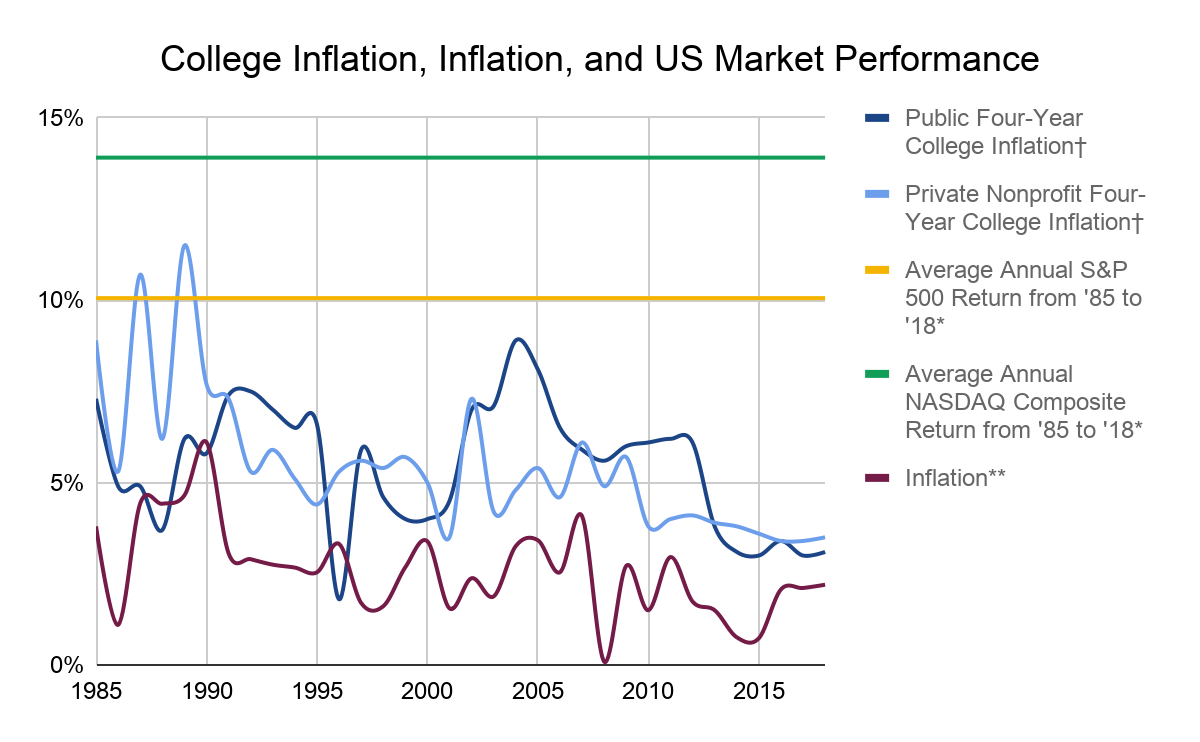
\includegraphics[width=\textwidth]{imgs/2.png}
    \caption{Time to plan the most important monetary investment in your children}
\end{figure}

\vspace{10pt}

\begin{figure}[!htb]
    \centering
    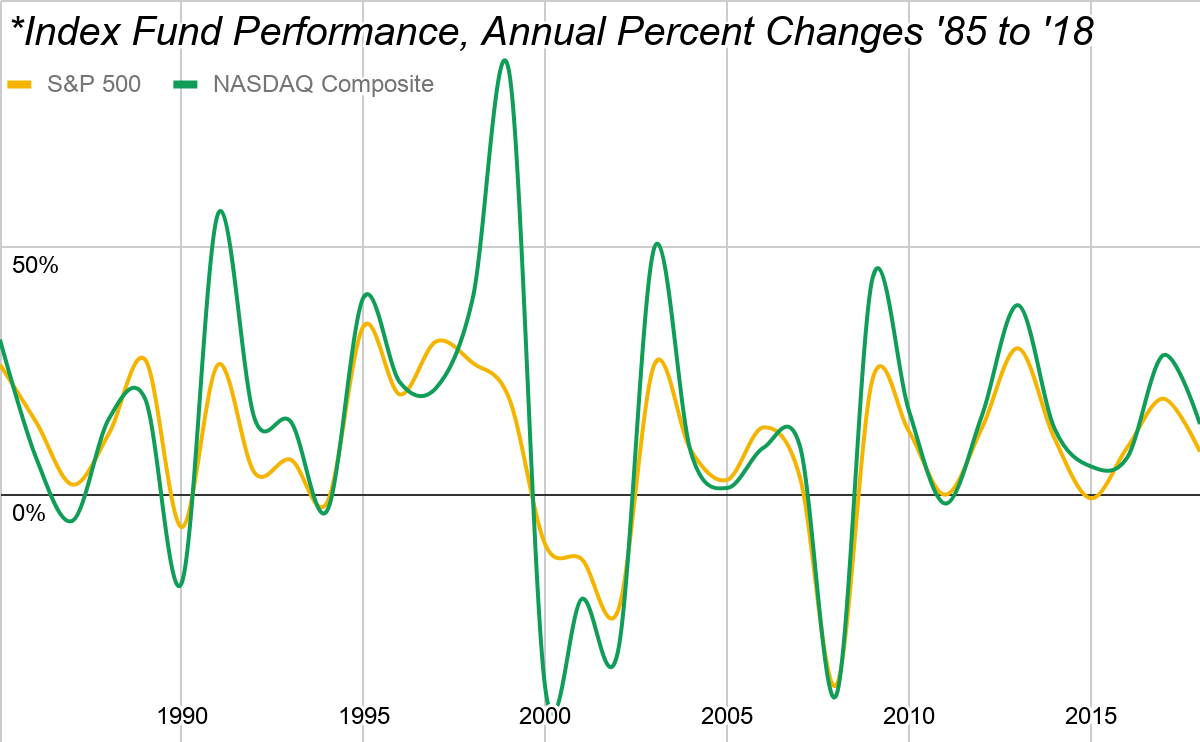
\includegraphics[width=\textwidth]{imgs/3.png}
    \caption{Top market indices}
\end{figure}

\vspace{10pt}

\begin{figure}[!htb]
    \centering
    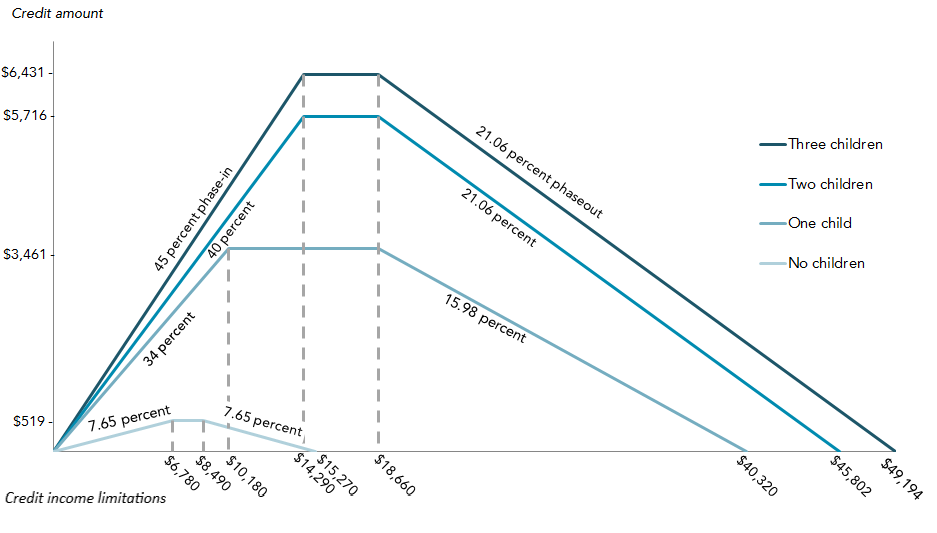
\includegraphics[width=\textwidth]{imgs/4.png}
    \caption{Earned Income Tax Credit bracket at the time}
\end{figure}

\vspace{10pt}

\begin{figure}[!htb]
    \centering
    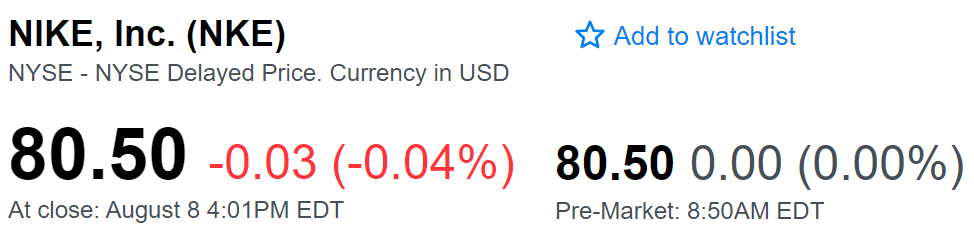
\includegraphics[width=\textwidth]{imgs/5.png}
    \caption{Basic stock quote}
\end{figure}

\clearpage
\vspace*{1in}

\begin{figure}[!htb]
    \centering
    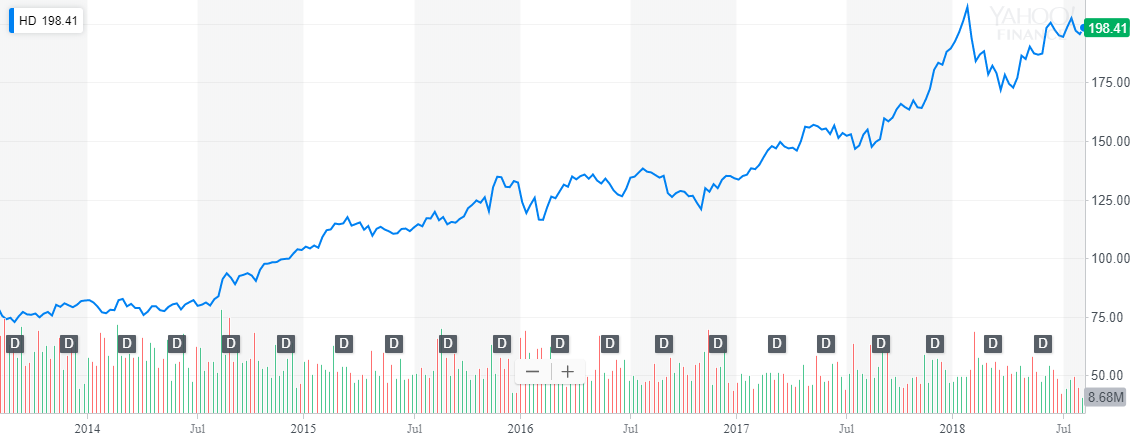
\includegraphics[width=\textwidth]{imgs/6.png}
    \caption{Basic stock price chart}
\end{figure}

\vspace{10pt}

\begin{figure}[!htb]
    \centering
    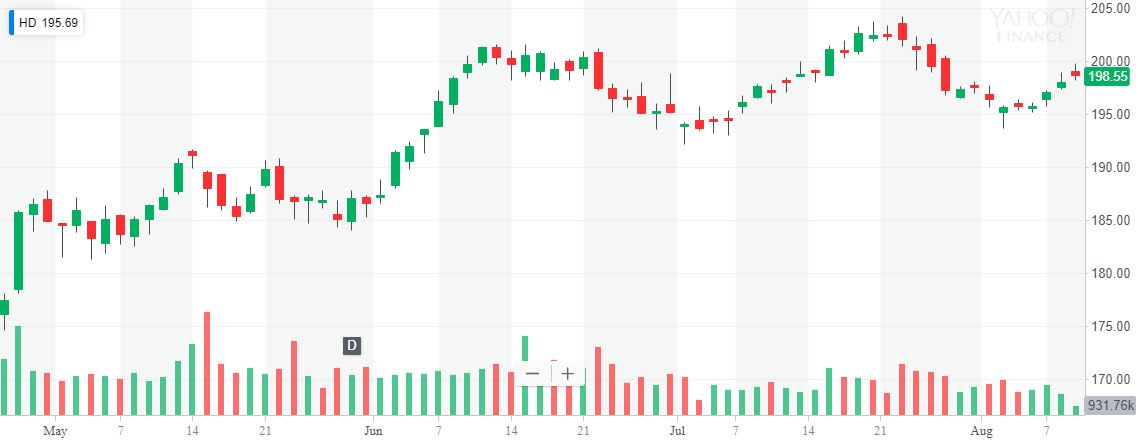
\includegraphics[width=\textwidth]{imgs/7.png}
    \caption{Candlestick chart give your valuable information}
\end{figure}

\vspace{10pt}

\begin{figure}[!htb]
    \centering
    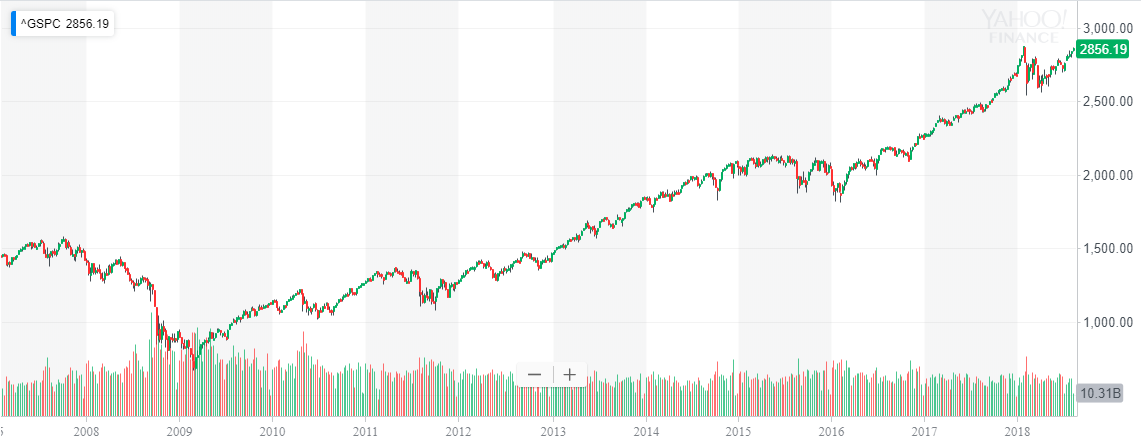
\includegraphics[width=\textwidth]{imgs/8.png}
    \caption{Stock index growth over time}
\end{figure}

\vspace{10pt}

\begin{figure}[!htb]
    \centering
    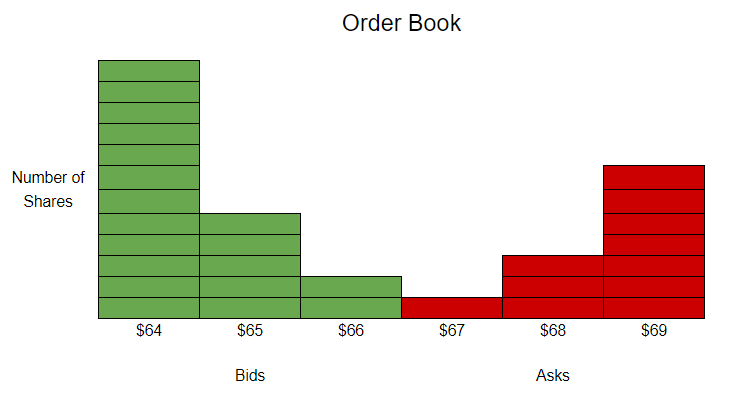
\includegraphics[width=\textwidth]{imgs/9.png}
    \caption{Simplified level 2 illustration}
\end{figure}

\vspace{10pt}

\begin{figure}[!htb]
    \centering
    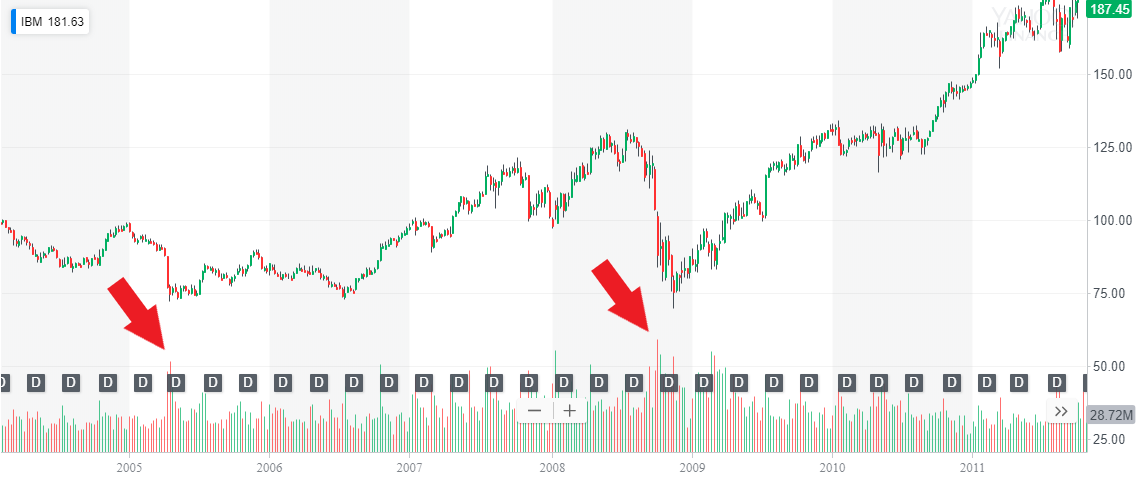
\includegraphics[width=\textwidth]{imgs/10.png}
    \caption{Big red volume bars}
\end{figure}

\vspace{10pt}

\begin{figure}[!htb]
    \centering
    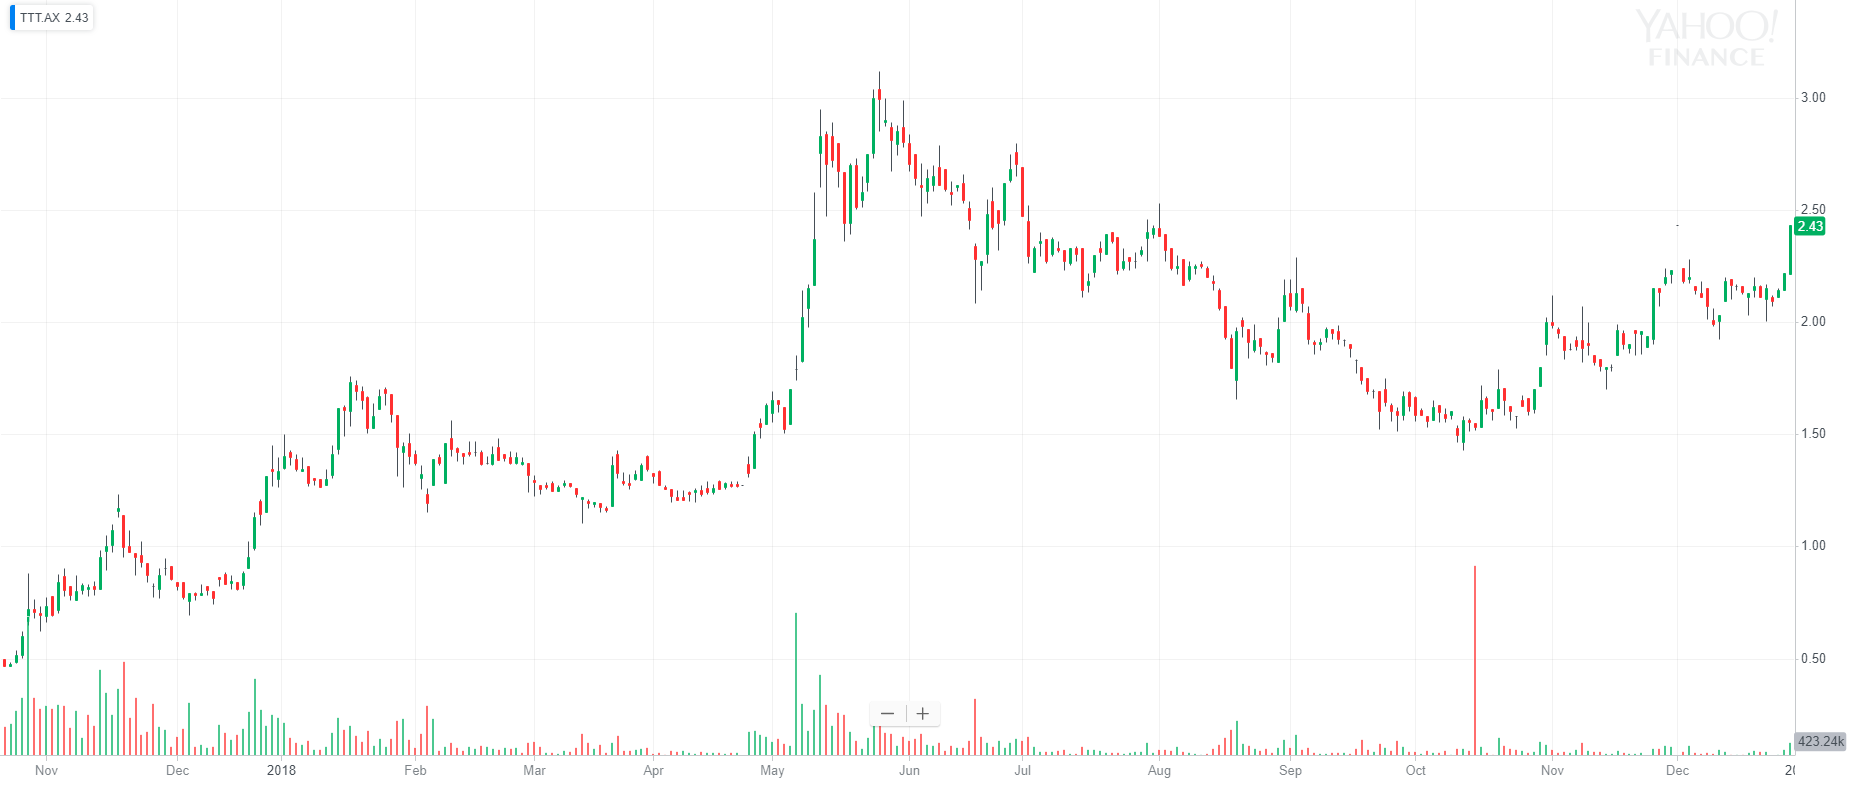
\includegraphics[width=\textwidth]{imgs/11.png}
    \caption{Consolidation and recovery}
\end{figure}

\vspace{10pt}

\begin{figure}[!htb]
    \centering
    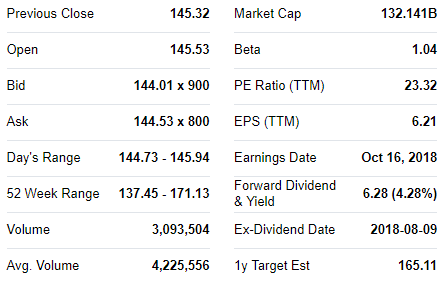
\includegraphics[width=.64\textwidth]{imgs/11.5.png}
    \caption{Key statistics}
\end{figure}

\vspace{10pt}

\begin{figure}[!htb]
    \centering
    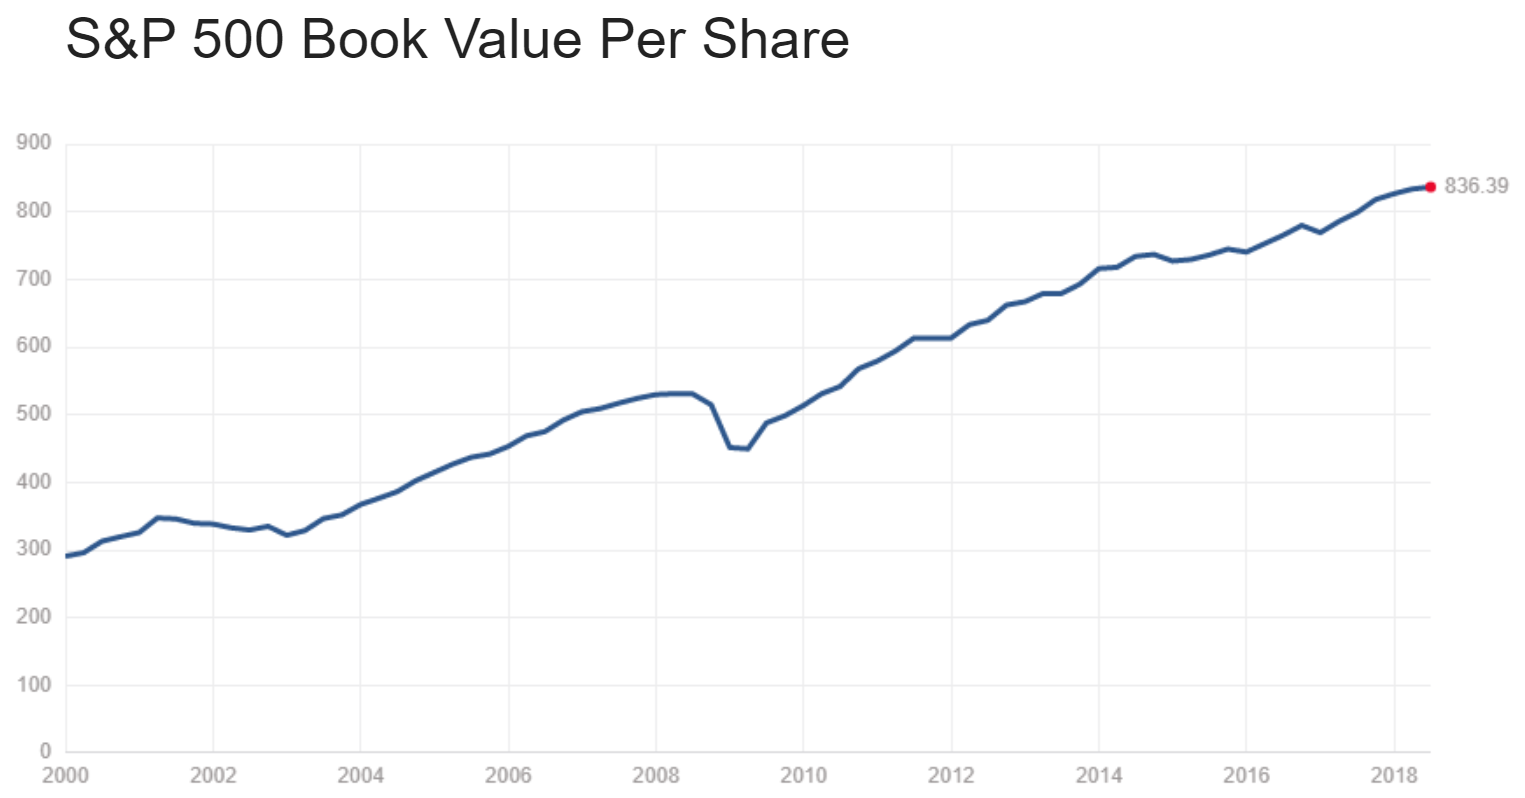
\includegraphics[width=\textwidth]{imgs/12.png}
    \caption{Fundamental value trends}
\end{figure}

\vspace{10pt}

\begin{figure}[!htb]
    \centering
    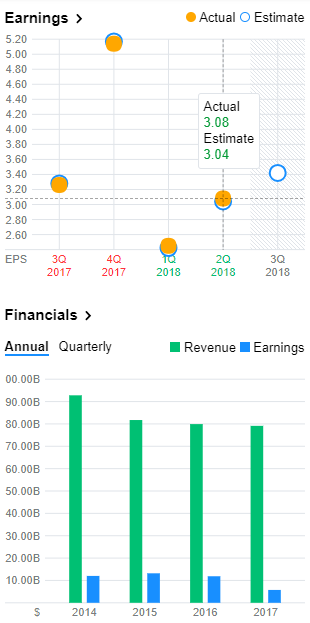
\includegraphics[width=.35\textwidth]{imgs/13.png}
    \caption{Yahoo Finance sidebar statistics}
\end{figure}

\vspace{10pt}

\begin{figure}[!htb]
    \centering
    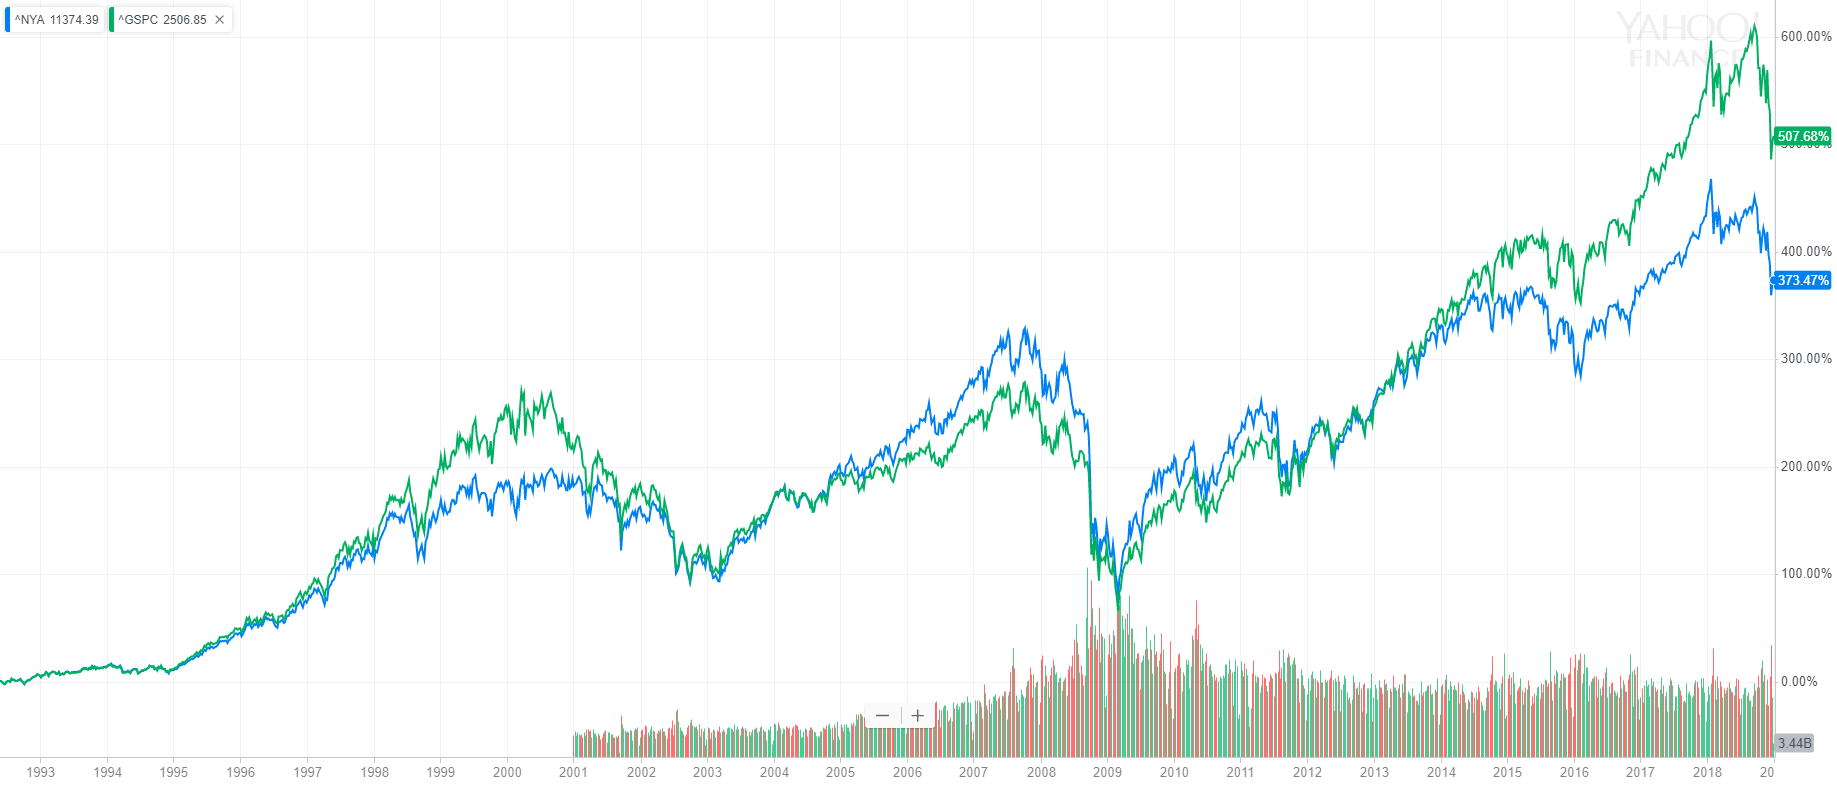
\includegraphics[width=\textwidth]{imgs/14.png}
    \caption{Overall comparison and insights}
\end{figure}

\vspace{10pt}

\begin{figure}[!htb]
    \centering
    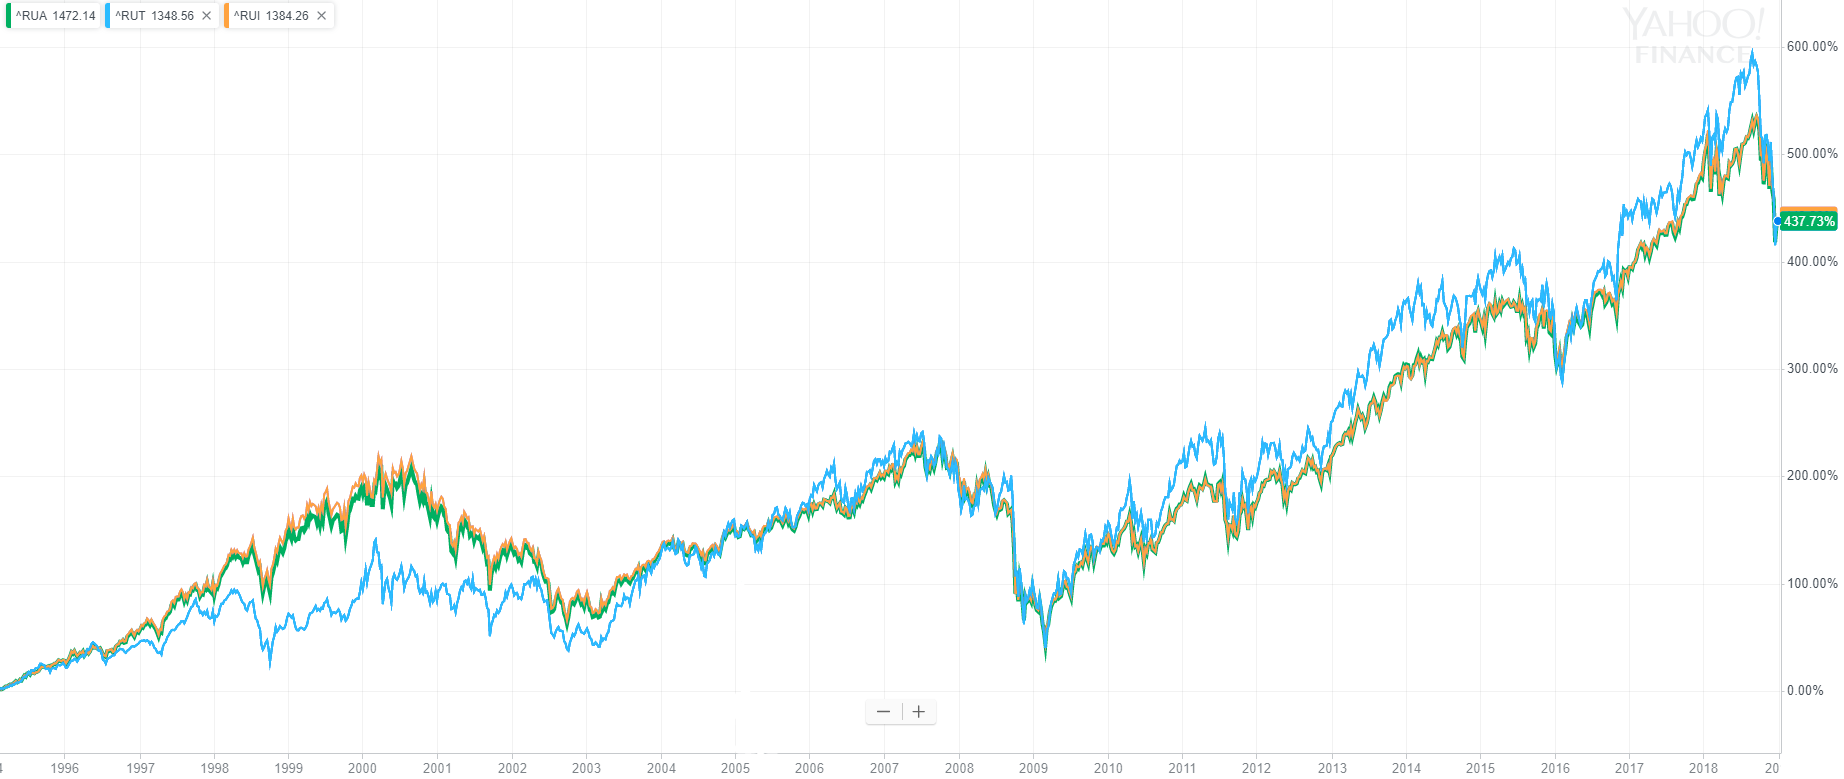
\includegraphics[width=\textwidth]{imgs/15.png}
    \caption{Additional factors to consider}
\end{figure}

\vspace{10pt}

\begin{figure}[!htb]
    \centering
    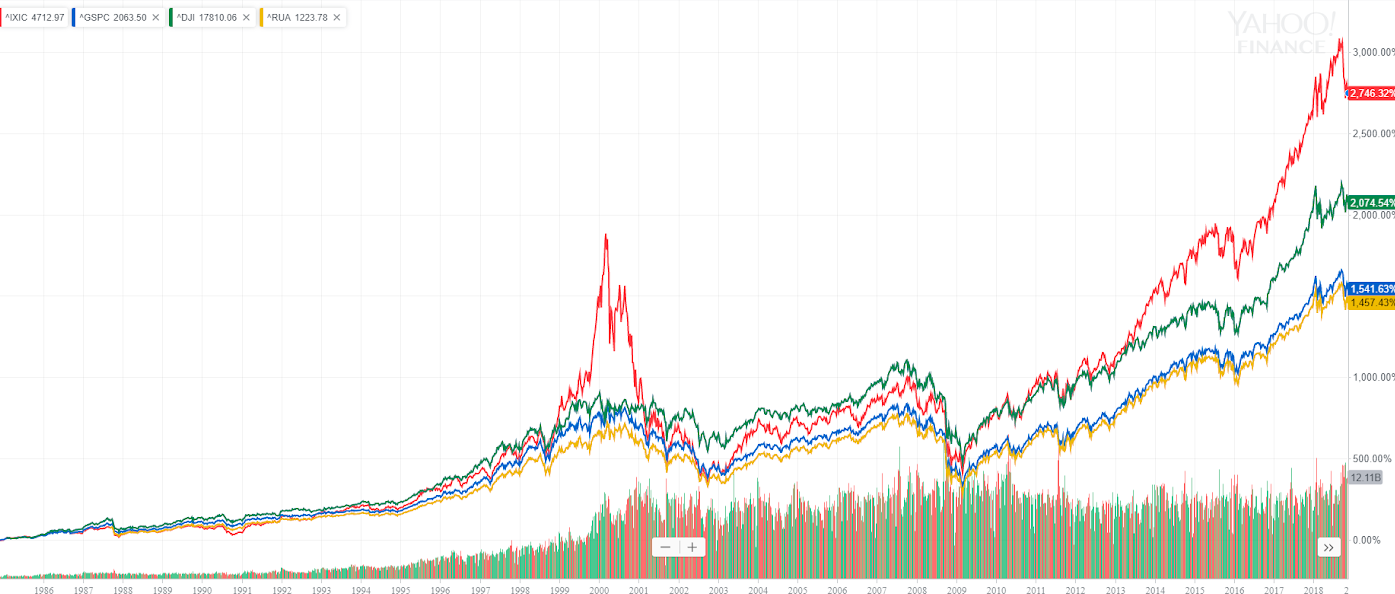
\includegraphics[width=\textwidth]{imgs/16.png}
    \caption{Volatility comparisons and risk introduction}
\end{figure}

\vspace{10pt}

\begin{figure}[!htb]
    \centering
    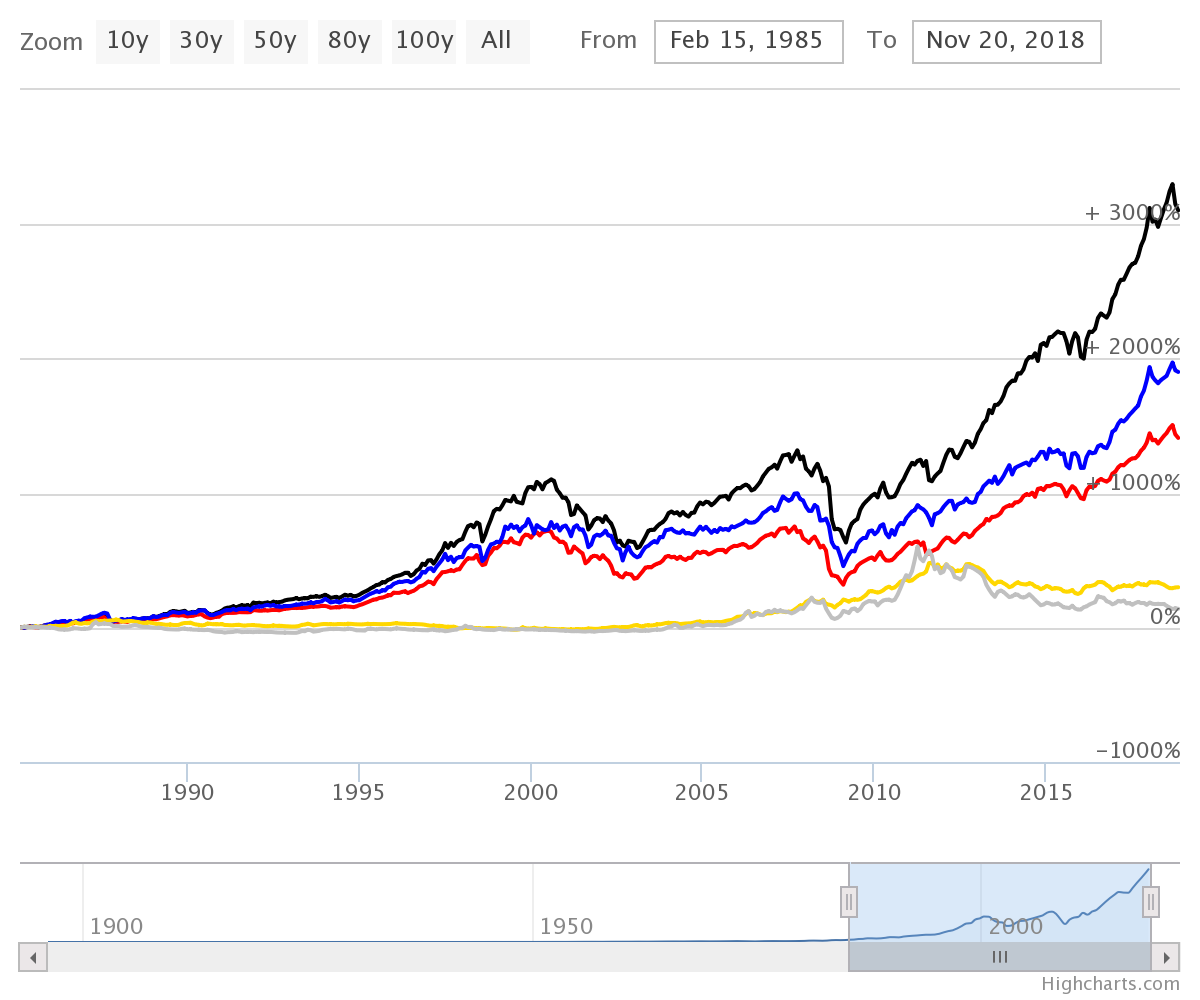
\includegraphics[width=450pt]{imgs/17.png}
    \caption{Nominal returns}
\end{figure}

\vspace{10pt}

\begin{figure}[!htb]
    \centering
    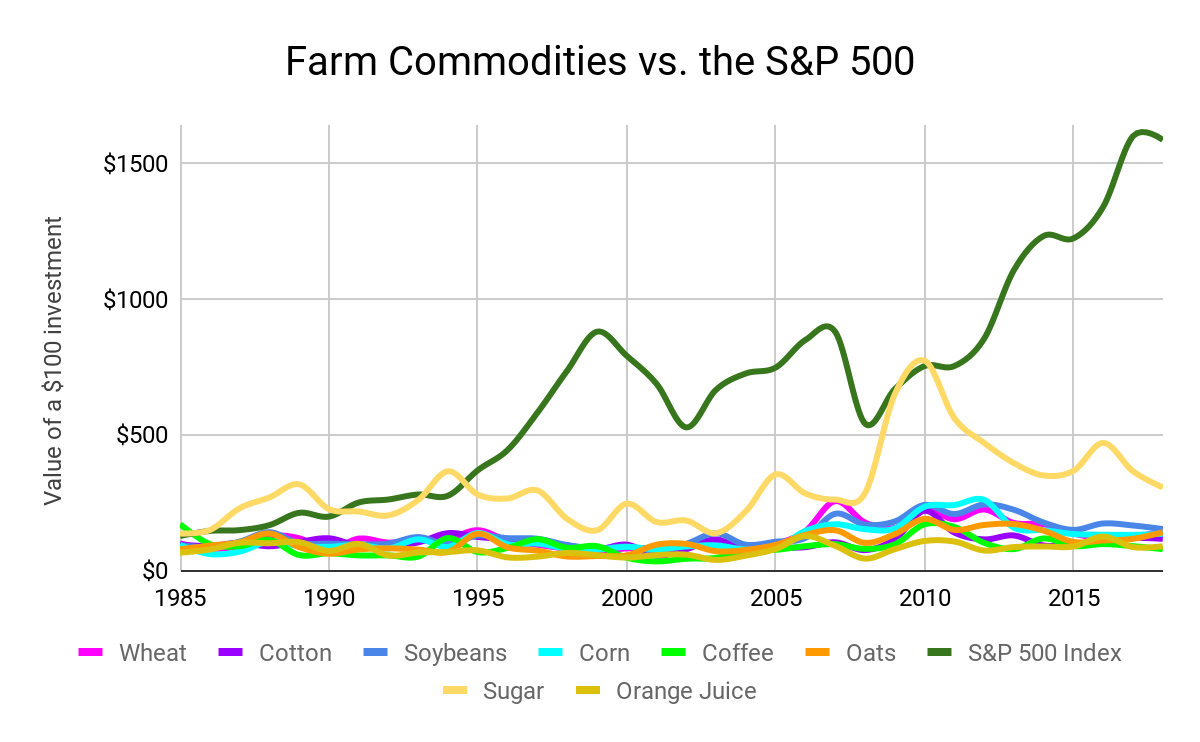
\includegraphics[width=\textwidth]{imgs/18.png}
    \caption{Long-term commodity trends, in fiat}
\end{figure}

\vspace{10pt}

\begin{figure}[!htb]
    \centering
    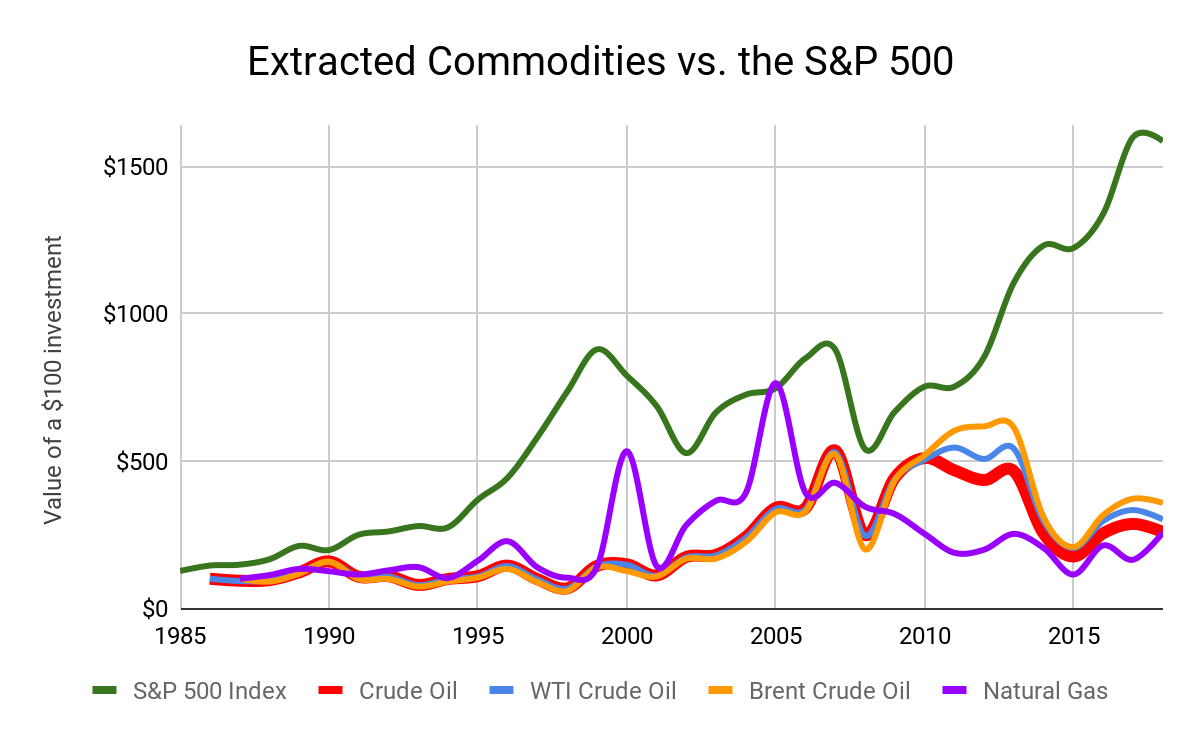
\includegraphics[width=\textwidth]{imgs/19.png}
    \caption{Energy sources contrasted}
\end{figure}

\vspace{10pt}

\begin{figure}[!htb]
    \centering
    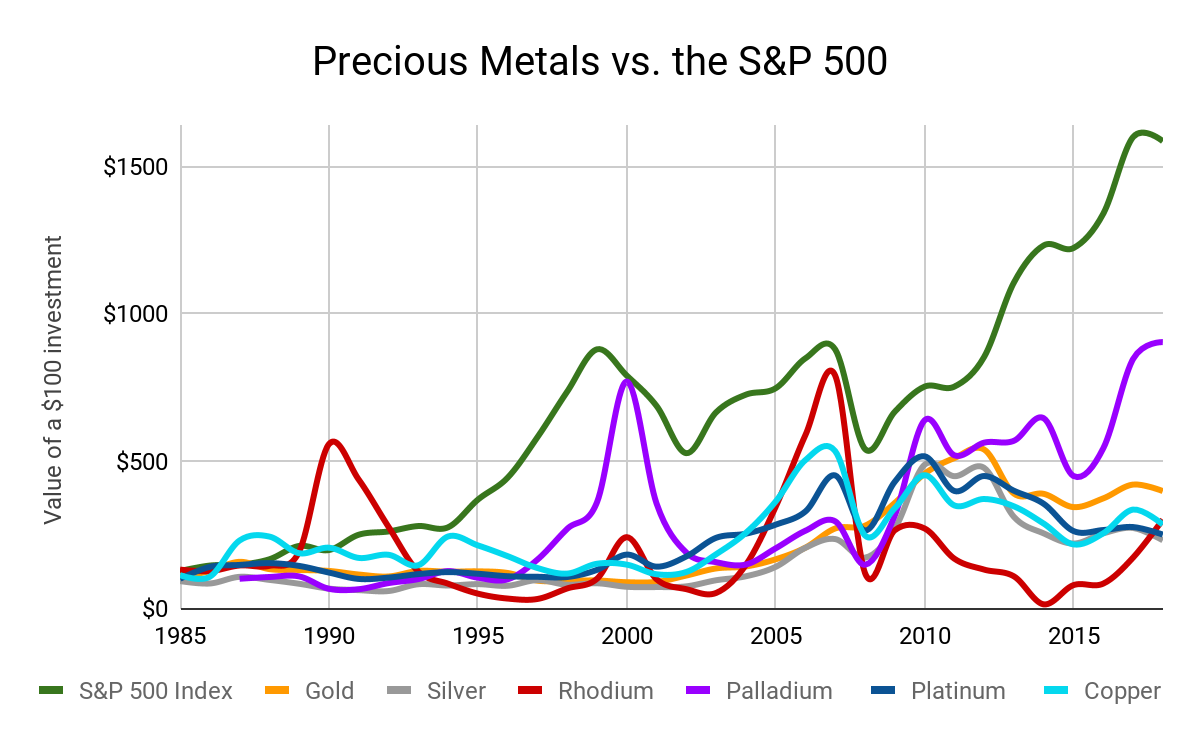
\includegraphics[width=\textwidth]{imgs/20.png}
    \caption{Metals values and trend insights, in fiat}
\end{figure}

\vspace{10pt}

\begin{figure}[!htb]
    \centering
    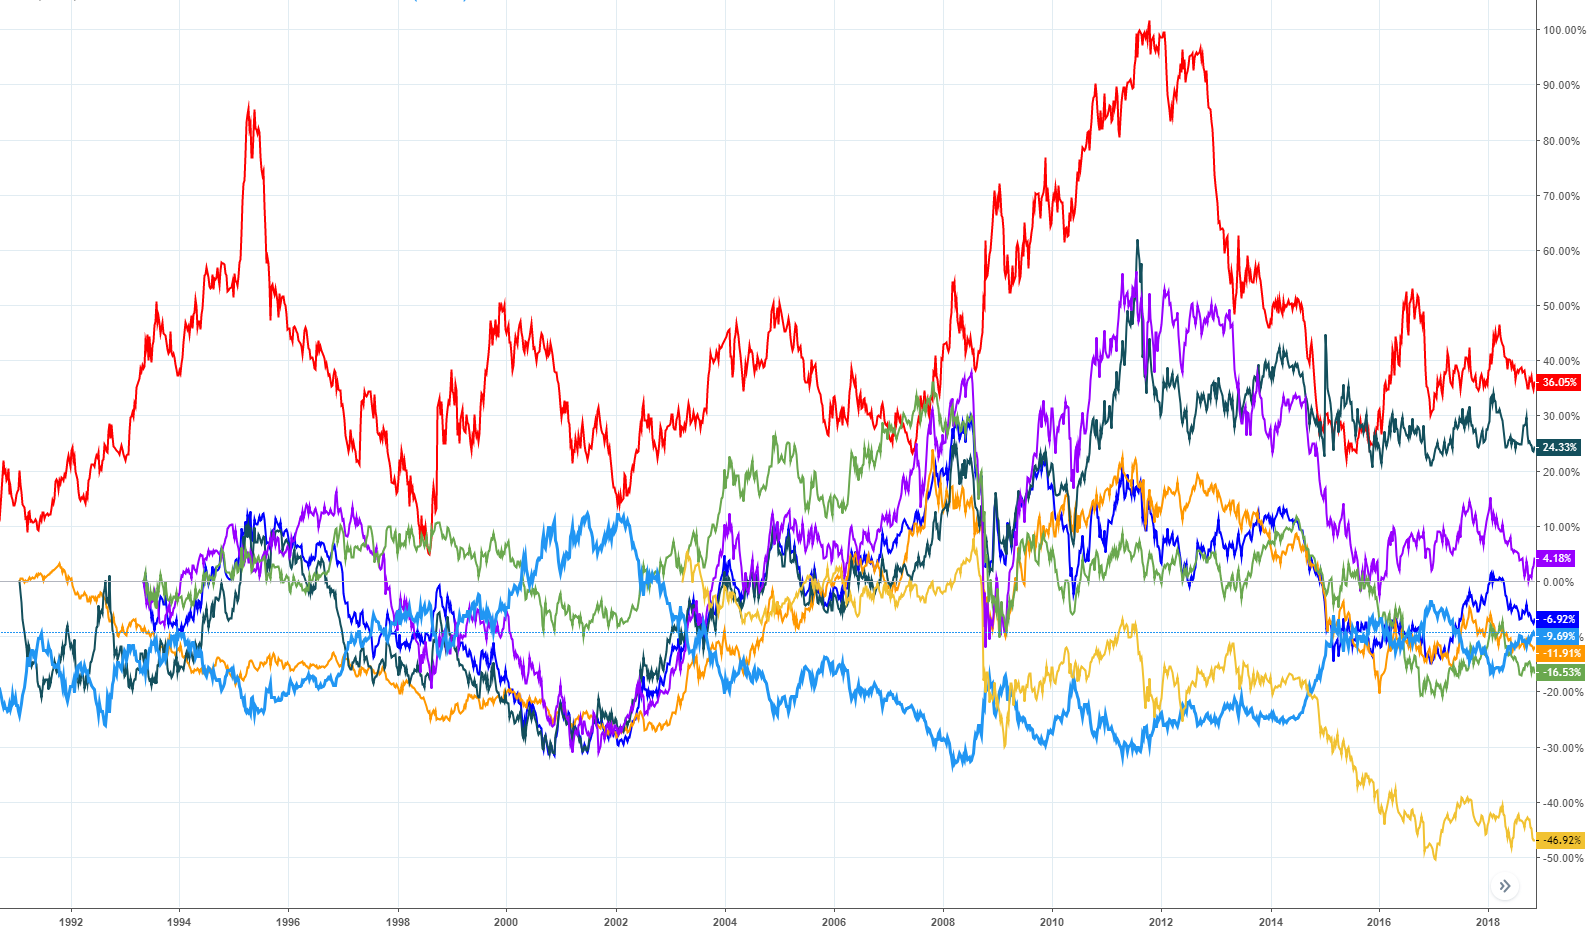
\includegraphics[width=\textwidth]{imgs/21.png}
    \caption{Introducing percent-based trend comparisons}
\end{figure}

\vspace{10pt}

\begin{figure}[!htb]
    \centering
    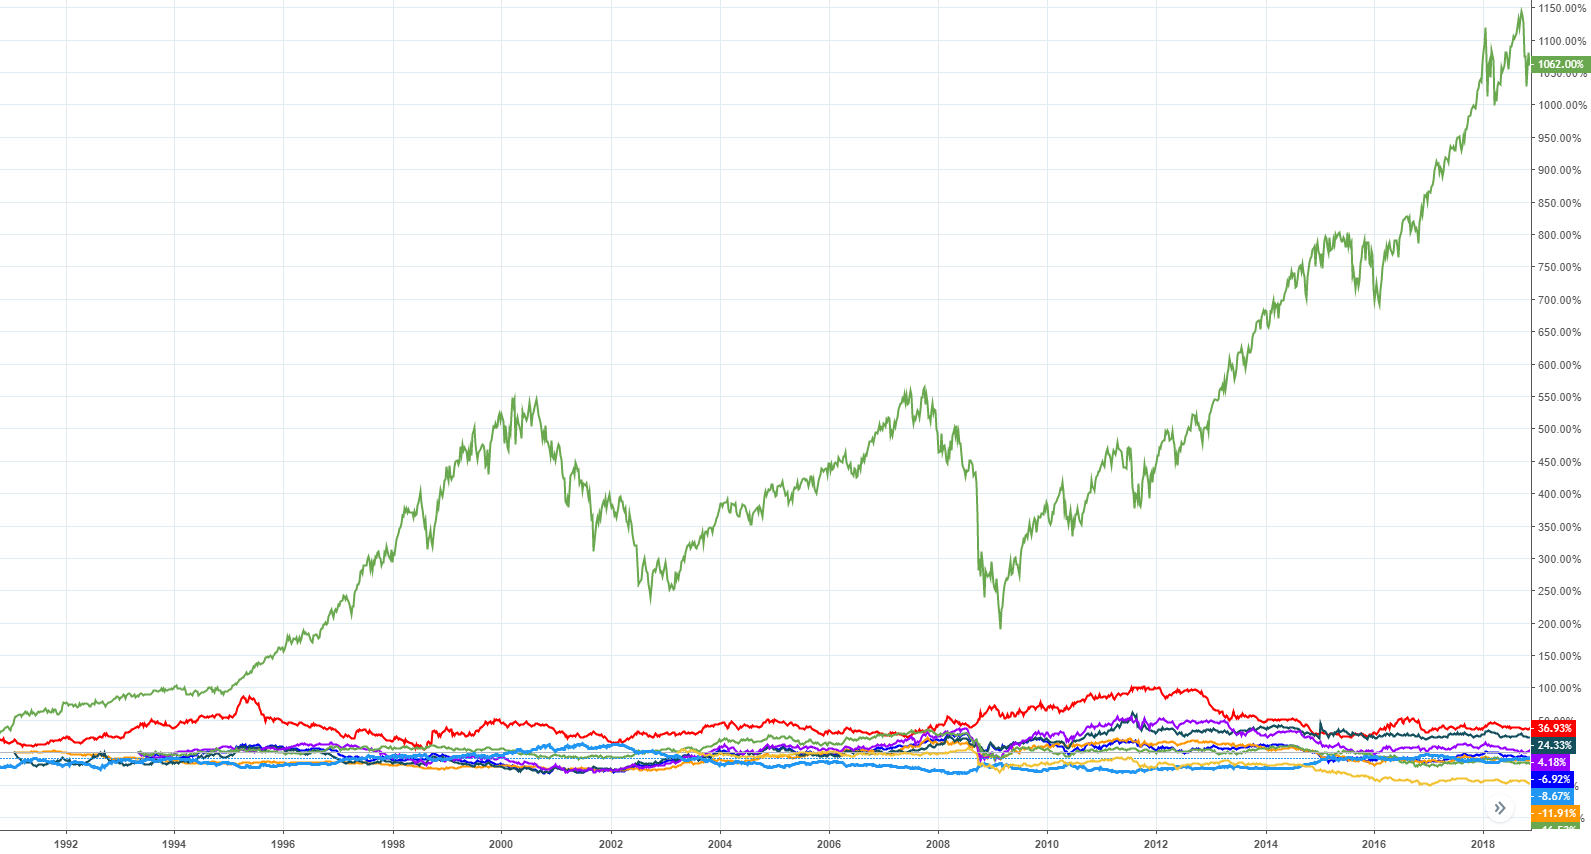
\includegraphics[width=\textwidth]{imgs/22.png}
    \caption{Equity market comparison}
\end{figure}

\vspace{10pt}

\begin{figure}[!htb]
    \centering
    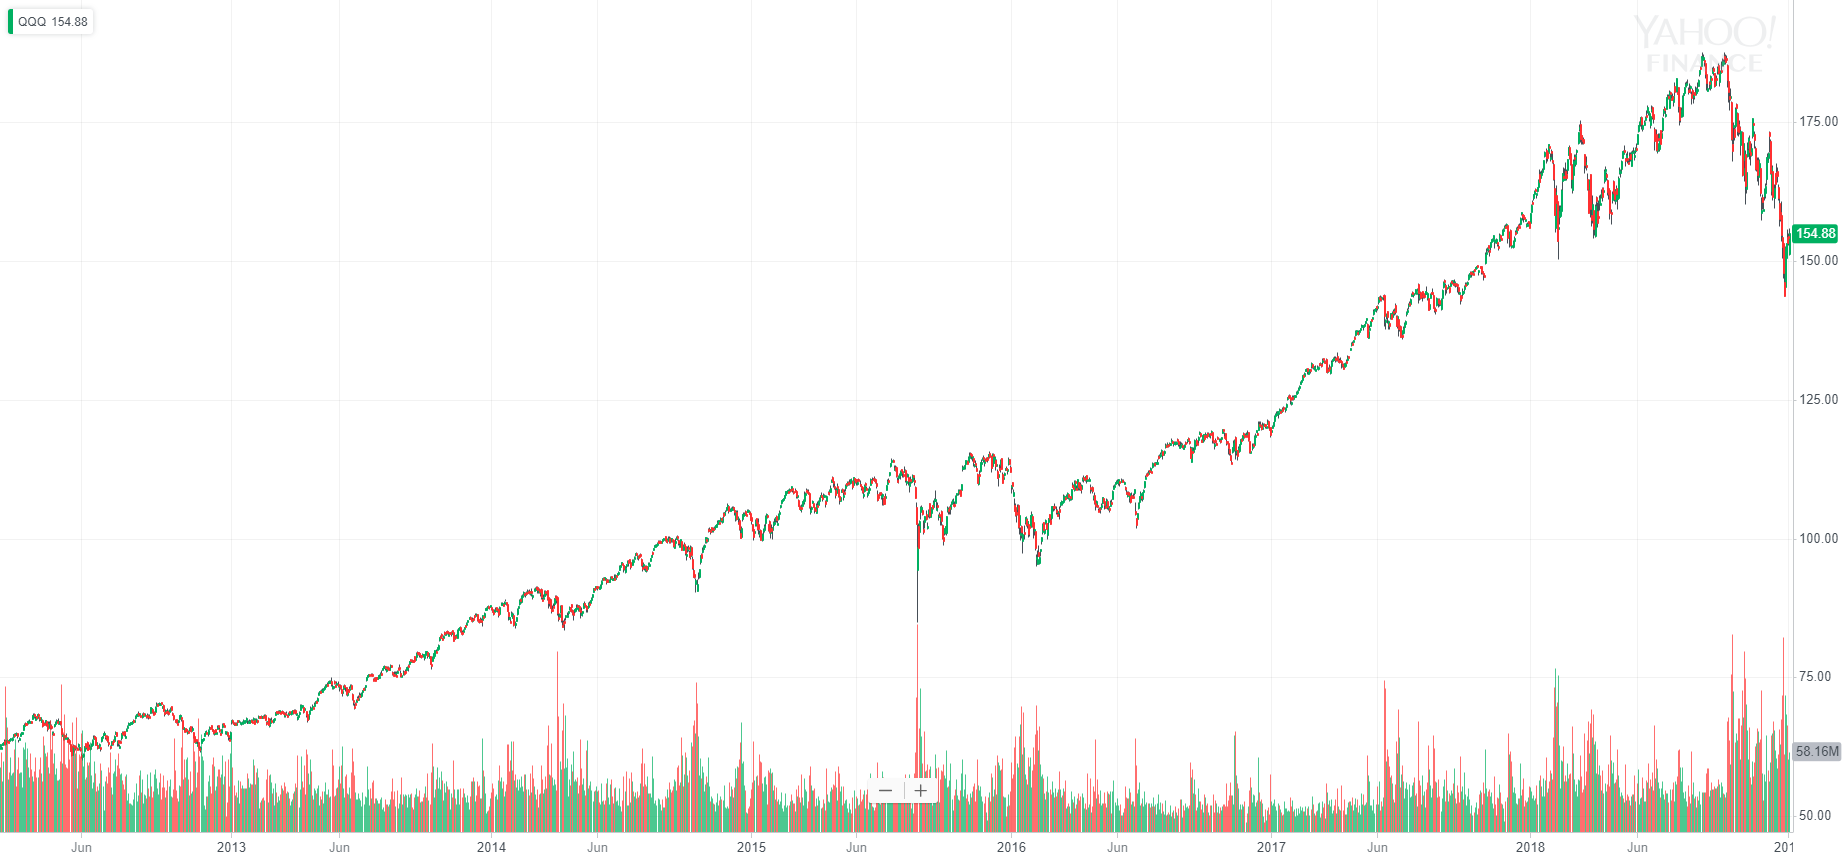
\includegraphics[width=\textwidth]{imgs/23.png}
    \caption{Options introduction and equity liquidity}
\end{figure}

\vspace{10pt}

\begin{figure}[!htb]
    \centering
    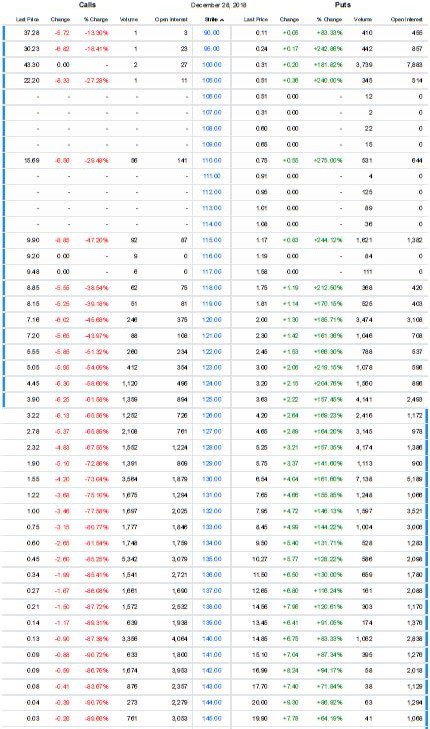
\includegraphics[width=.42\textwidth]{imgs/24.png}
    \caption{Options chain and insights}
\end{figure}

\vspace{10pt}

\begin{figure}[!htb]
    \centering
    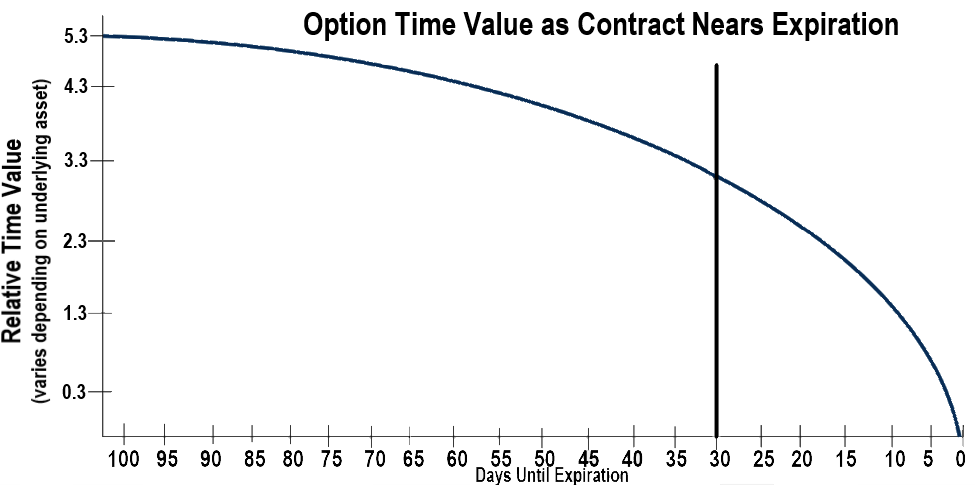
\includegraphics[width=\textwidth]{imgs/25.png}
    \caption{External contract value added and trading considerations}
\end{figure}

\vspace{10pt}

\begin{figure}[!htb]
    \centering
    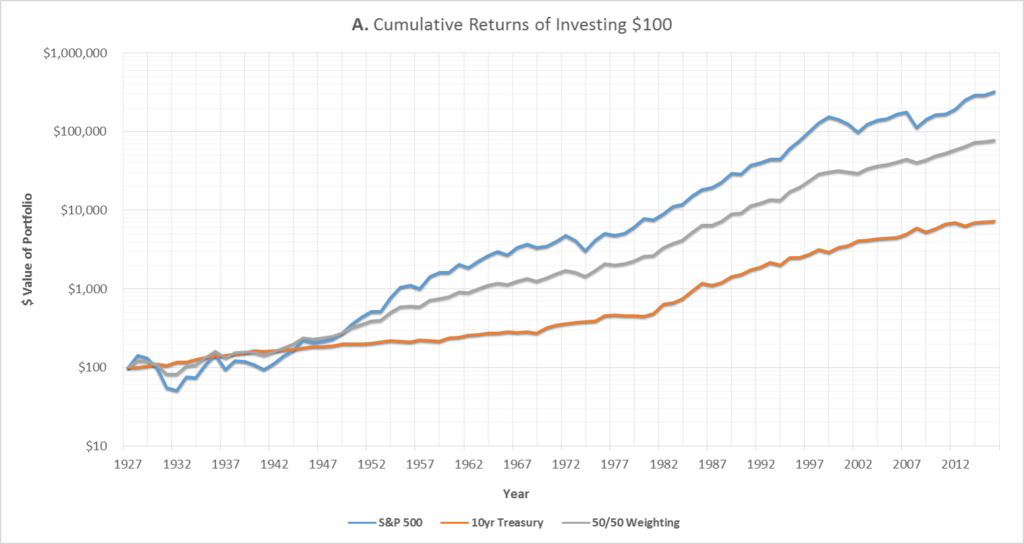
\includegraphics[width=\textwidth]{imgs/26.png}
    \caption{Introducing bonds}
\end{figure}

\vspace{10pt}

\begin{figure}[!htb]
    \centering
    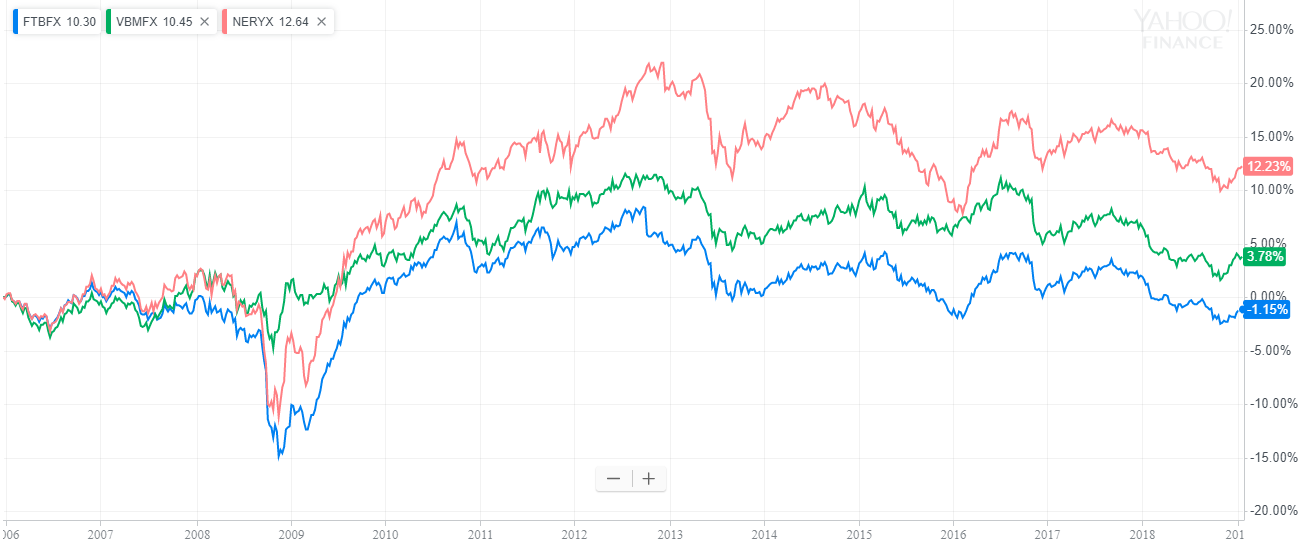
\includegraphics[width=\textwidth]{imgs/27.png}
    \caption{Select bond indices compared}
\end{figure}

\vspace{10pt}

\begin{figure}[!htb]
    \centering
    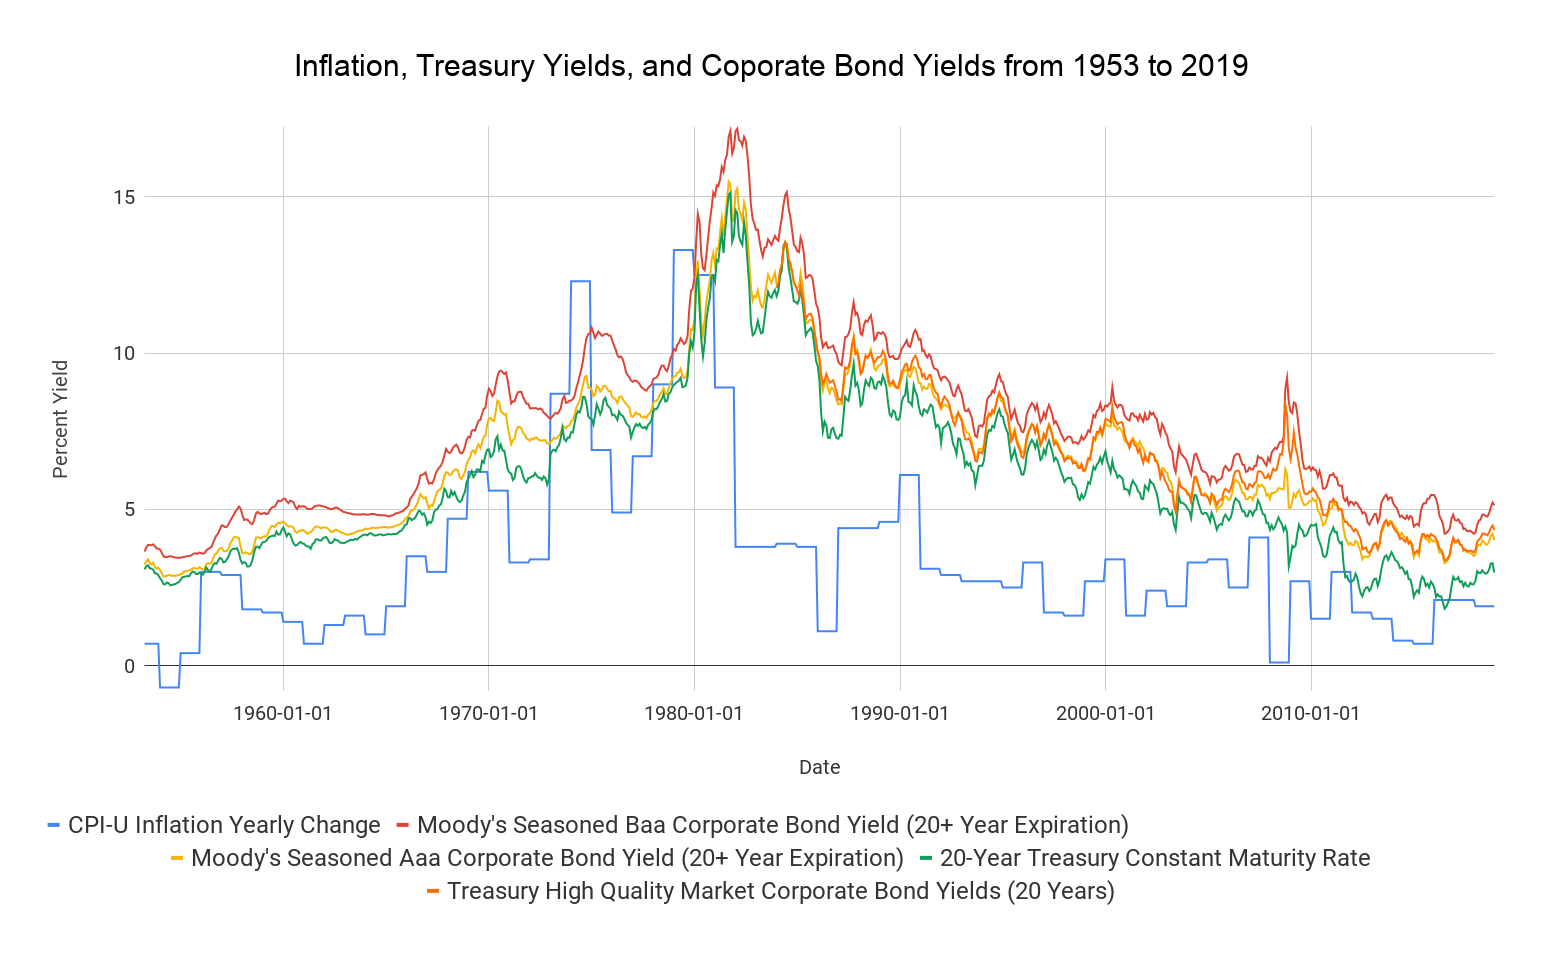
\includegraphics[width=\textwidth]{imgs/28.png}
    \caption{Real return considerations}
\end{figure}

\vspace{10pt}

\begin{figure}[!htb]
    \centering
    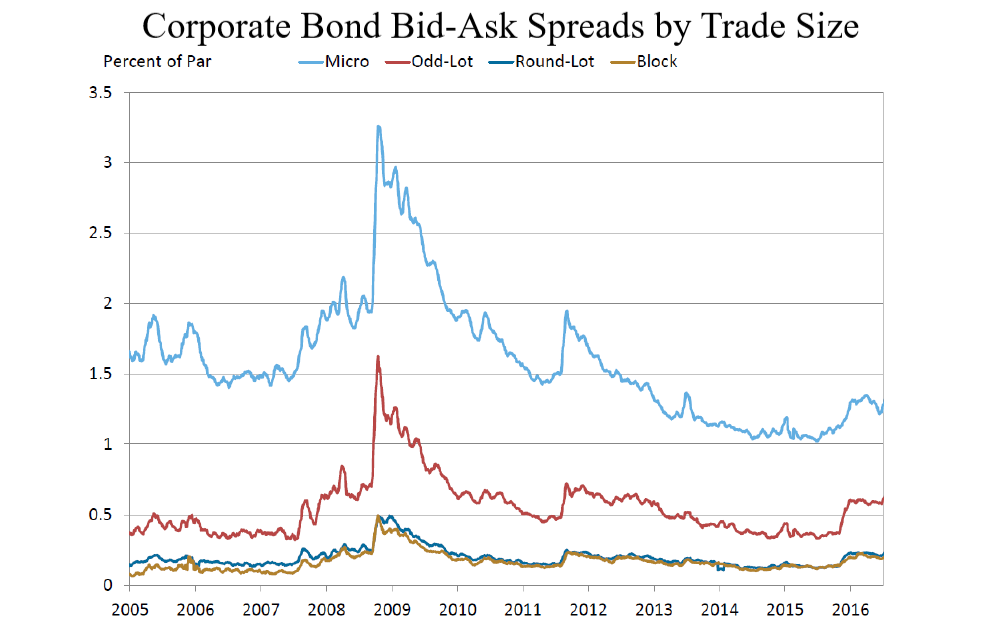
\includegraphics[width=\textwidth]{imgs/29.png}
    \caption{Practical trading factors}
\end{figure}

\vspace{10pt}

\begin{figure}[!htb]
    \centering
    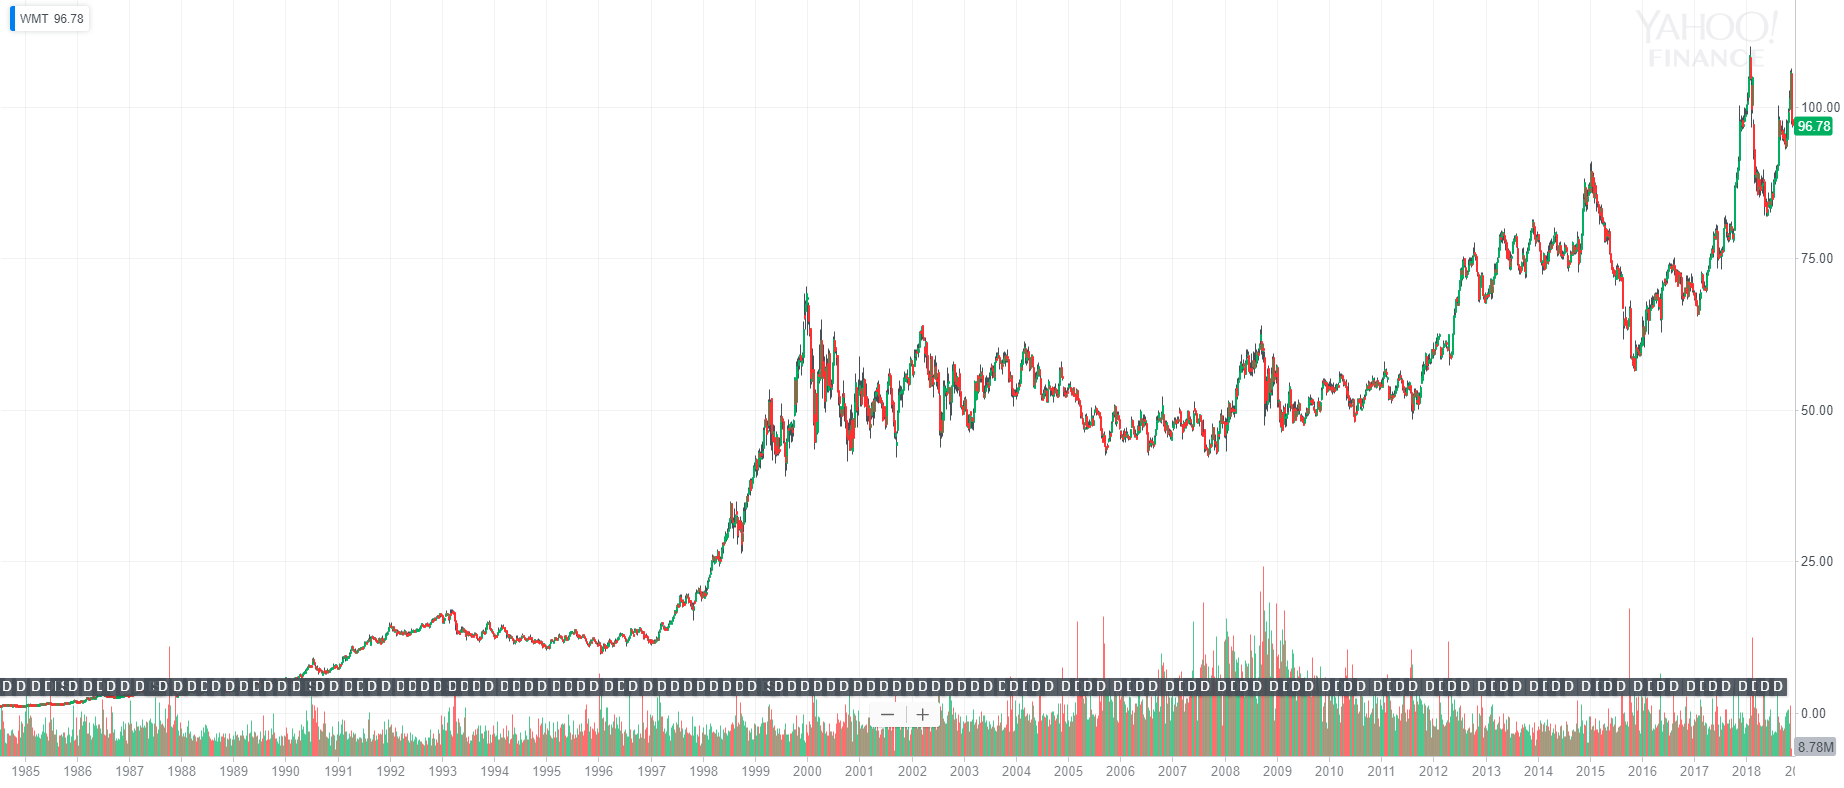
\includegraphics[width=\textwidth]{imgs/30.png}
    \caption{Dividends and their frequency}
\end{figure}

\vspace{10pt}

\begin{figure}[!htb]
    \centering
    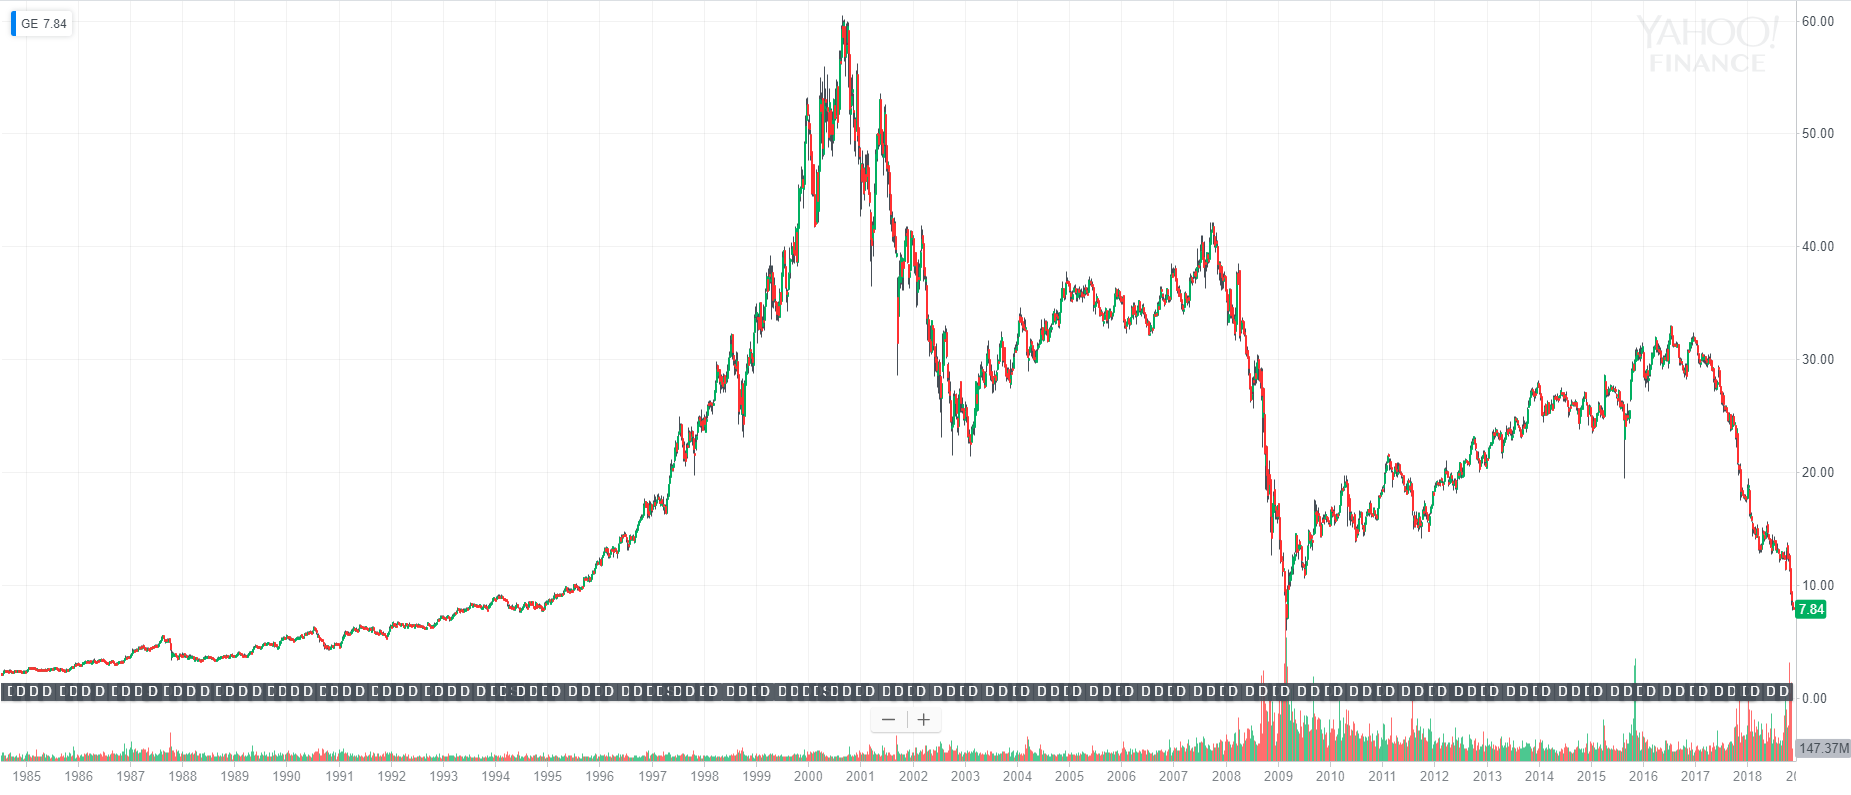
\includegraphics[width=\textwidth]{imgs/31.png}
    \caption{Impact in bear markets}
\end{figure}

\vspace{10pt}

\begin{figure}[!htb]
    \centering
    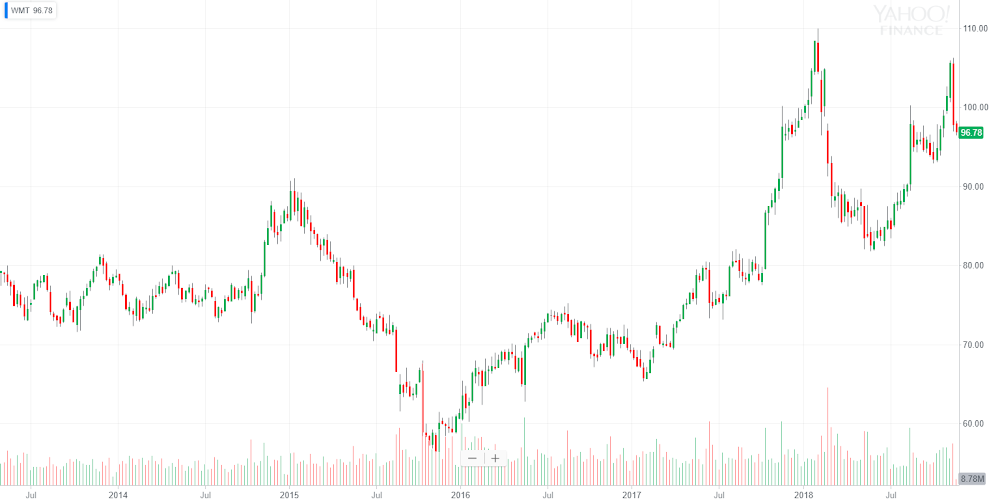
\includegraphics[width=\textwidth]{imgs/32.png}
    \caption{Affects considering technical analysis}
\end{figure}

\vspace{10pt}

\begin{figure}[!htb]
    \centering
    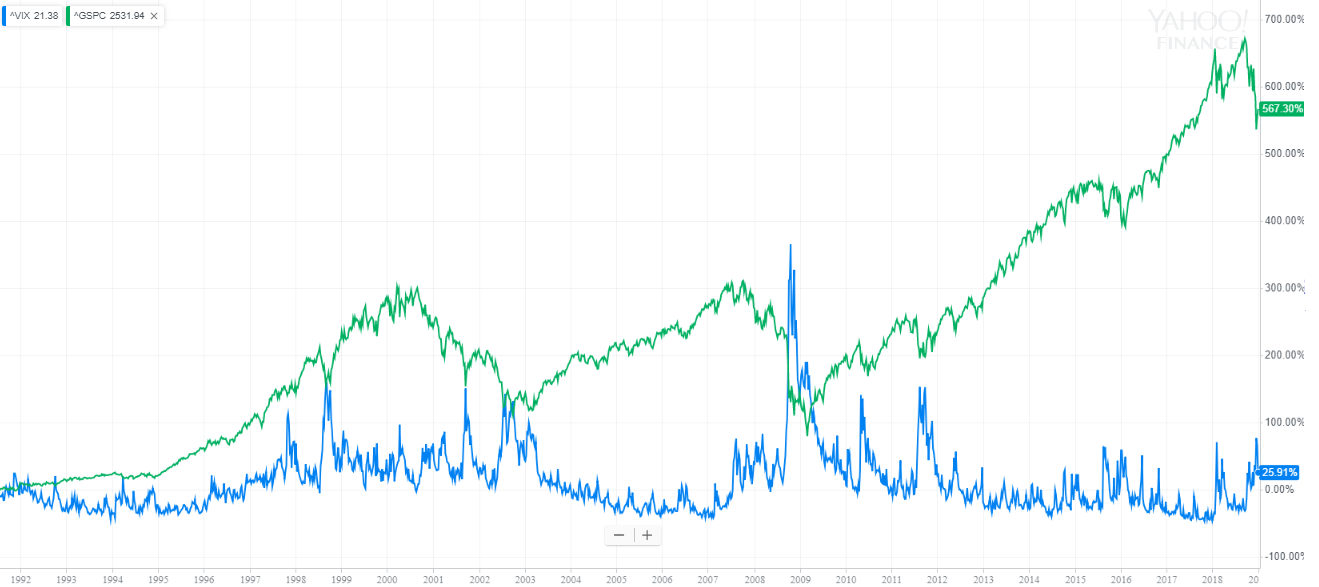
\includegraphics[width=\textwidth]{imgs/33.png}
    \caption{Inverse relationships}
\end{figure}

\vspace{10pt}

\begin{figure}[!htb]
    \centering
    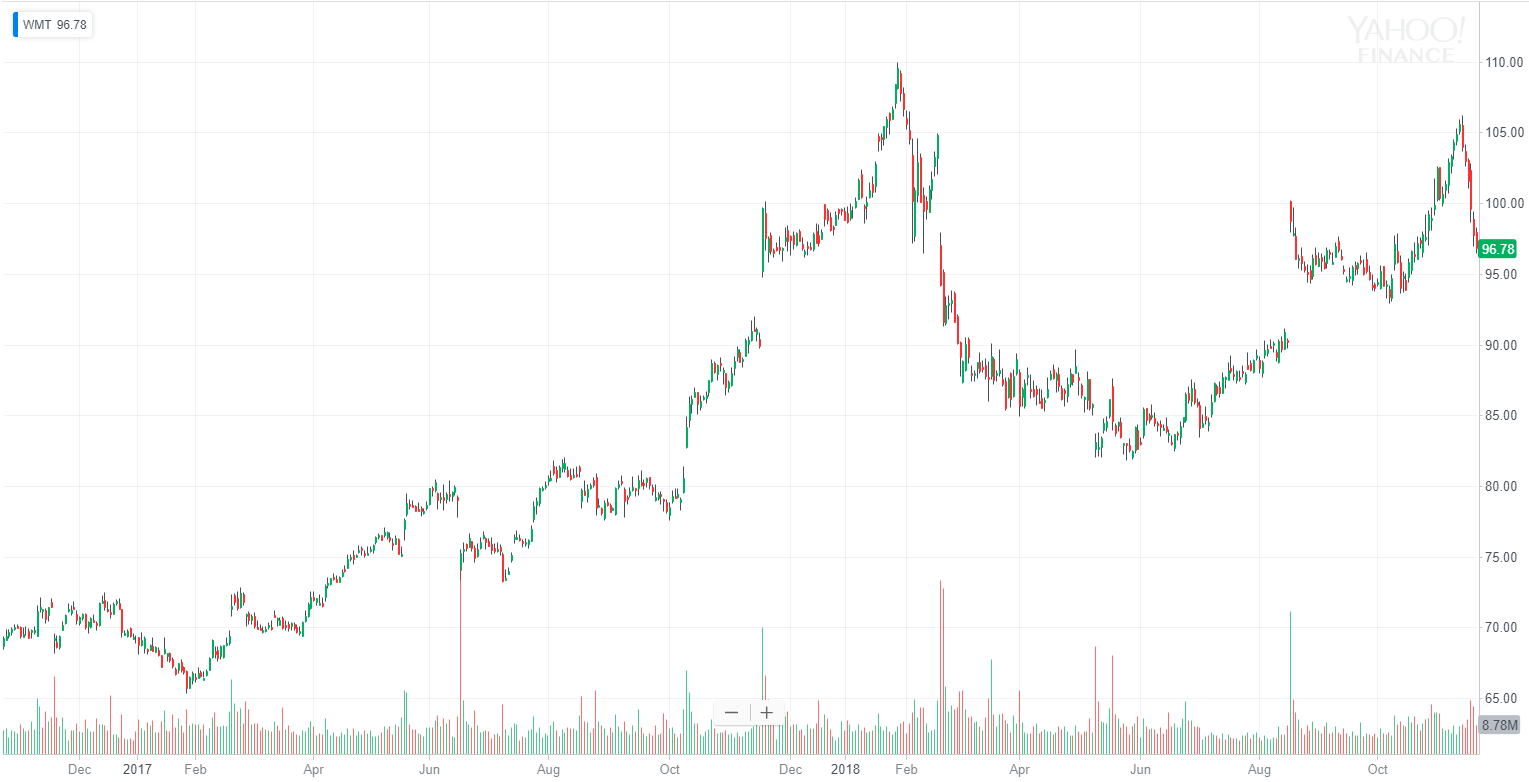
\includegraphics[width=\textwidth]{imgs/34.png}
    \caption{Trading haults and daily hour limitations and implications}
\end{figure}

\vspace{10pt}

\begin{figure}[!htb]
    \centering
    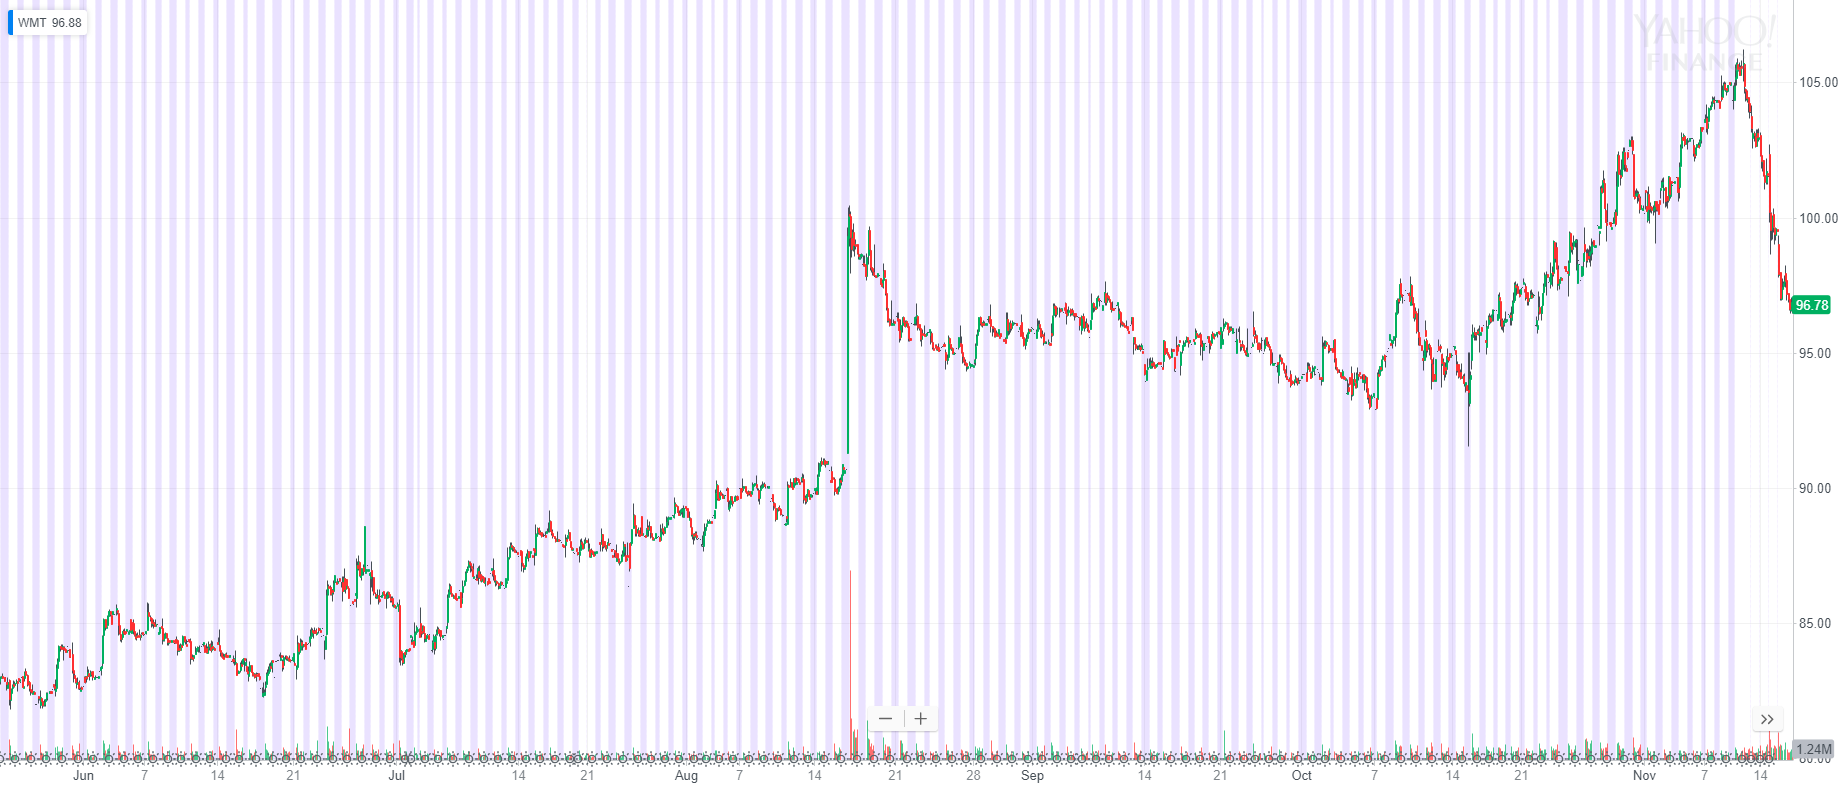
\includegraphics[width=\textwidth]{imgs/35.png}
    \caption{Introducing premarket gainers}
\end{figure}

\vspace{10pt}

\begin{figure}[!htb]
    \centering
    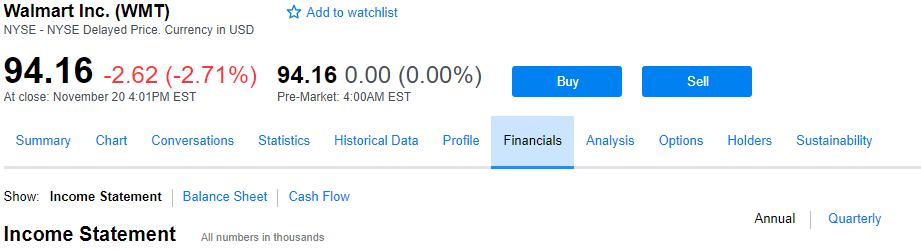
\includegraphics[width=\textwidth]{imgs/36.png}
    \caption{Standout financials}
\end{figure}

\vspace{10pt}

\begin{figure}[!htb]
    \centering
    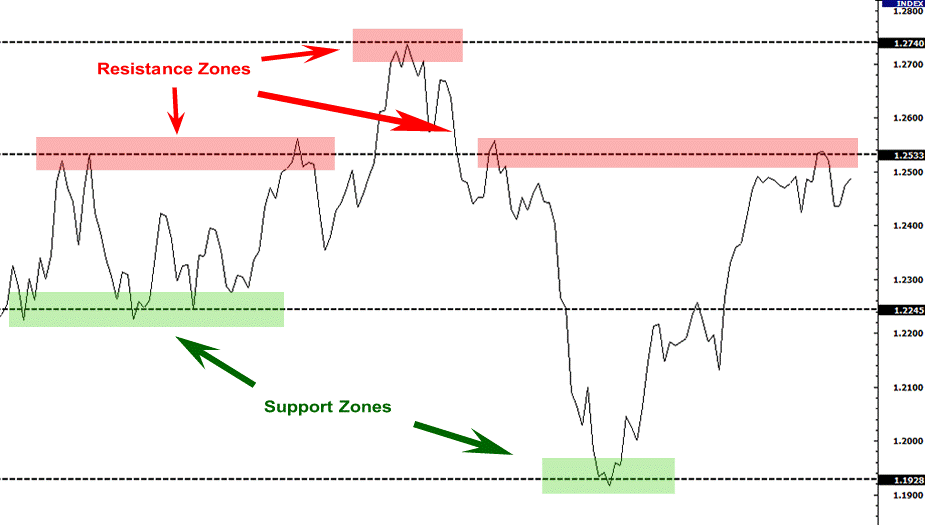
\includegraphics[width=\textwidth]{imgs/37.png}
    \caption{Support and resistance}
\end{figure}

\vspace{10pt}

\begin{figure}[!htb]
    \centering
    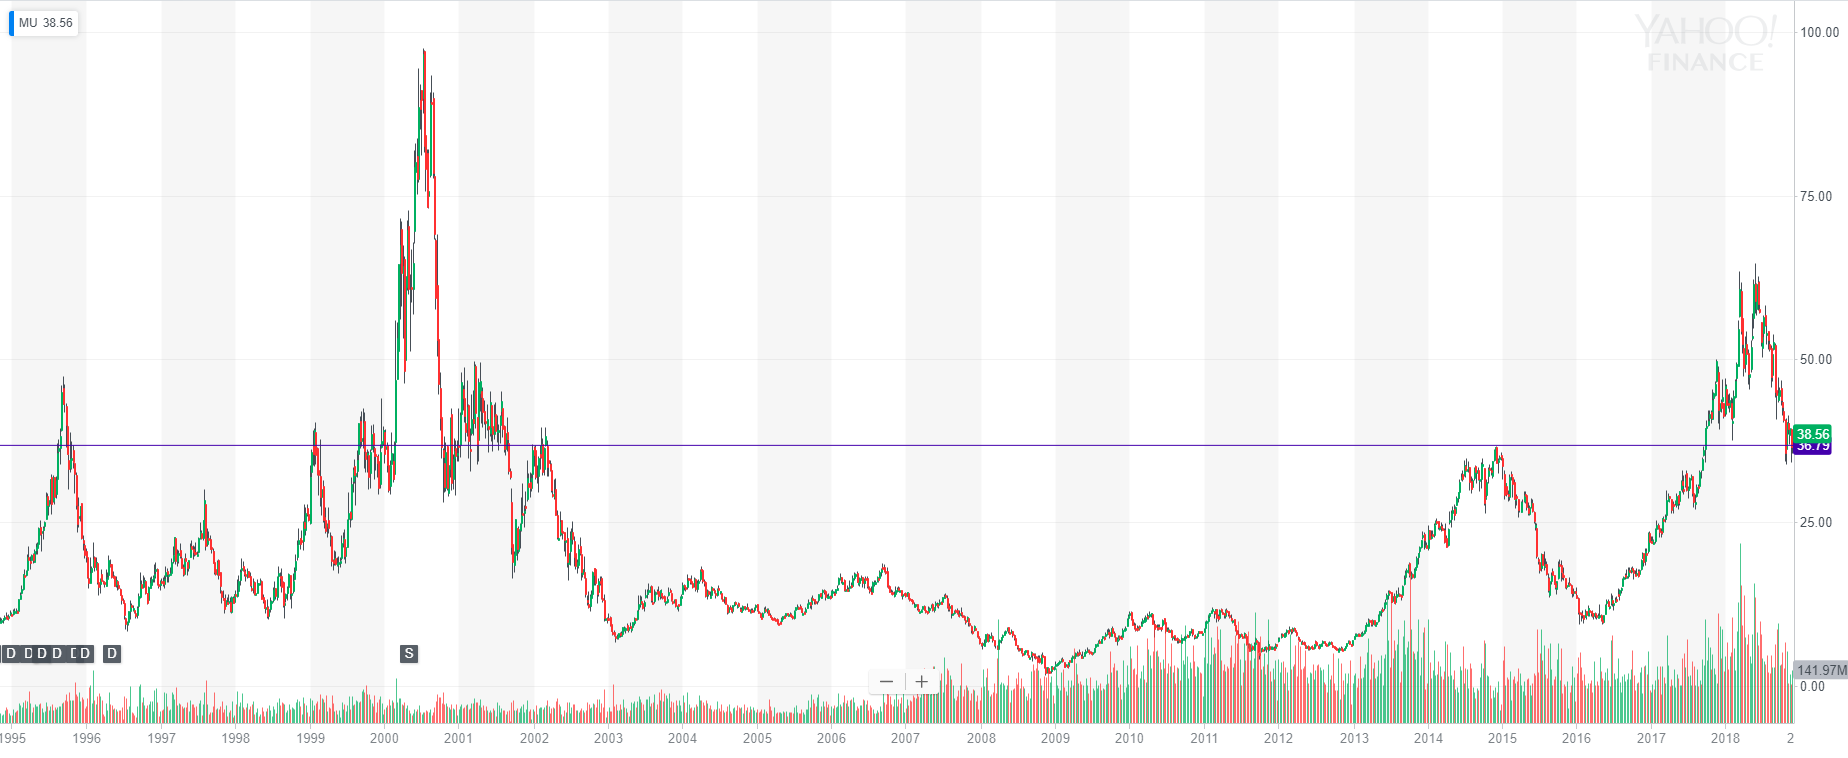
\includegraphics[width=\textwidth]{imgs/38.png}
    \caption{Example of a major price level}
\end{figure}

\vspace{10pt}

\begin{figure}[!htb]
    \centering
    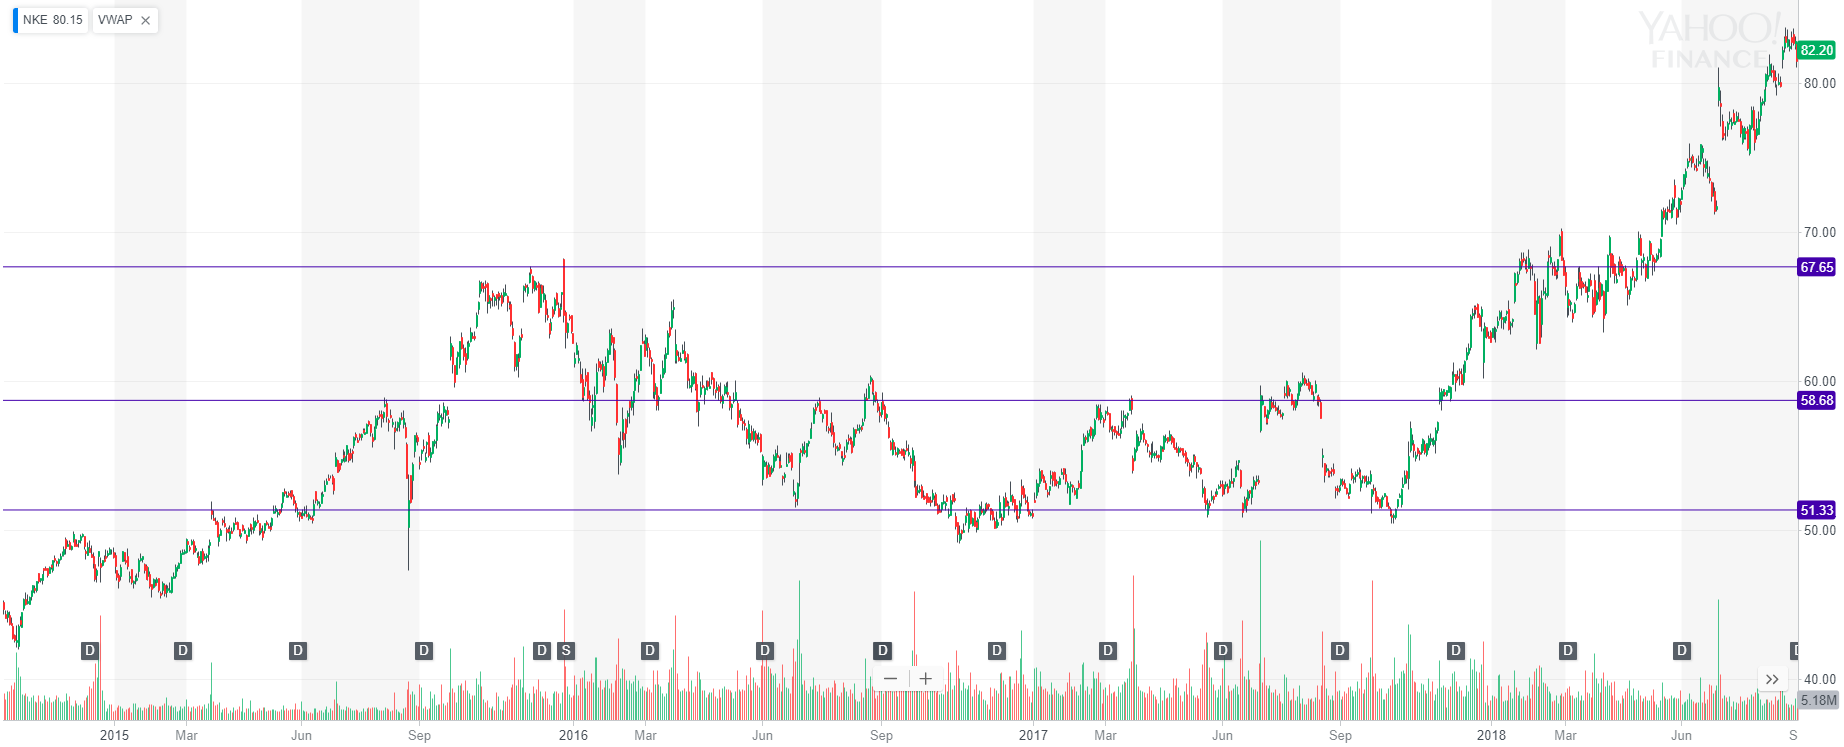
\includegraphics[width=\textwidth]{imgs/39.png}
    \caption{Diving into nuanced levels}
\end{figure}

\vspace{10pt}

\begin{figure}[!htb]
    \centering
    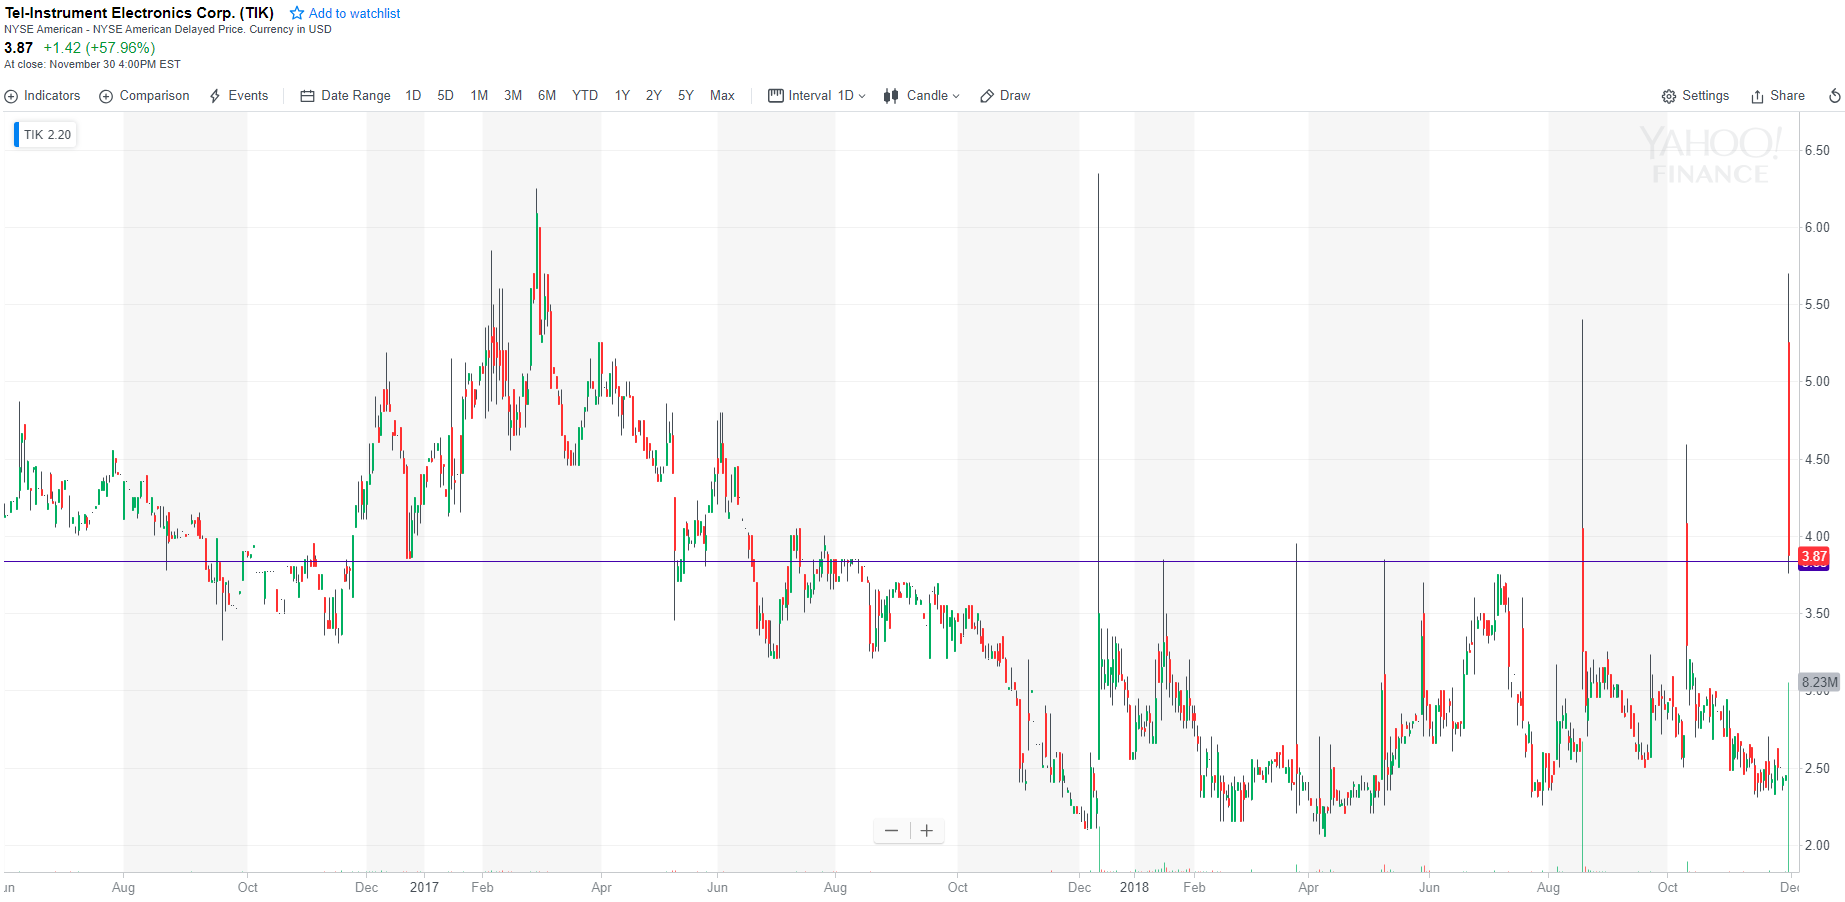
\includegraphics[width=\textwidth]{imgs/40.png}
    \caption{Price target implications}
\end{figure}

\vspace{10pt}

\begin{figure}[!htb]
    \centering
    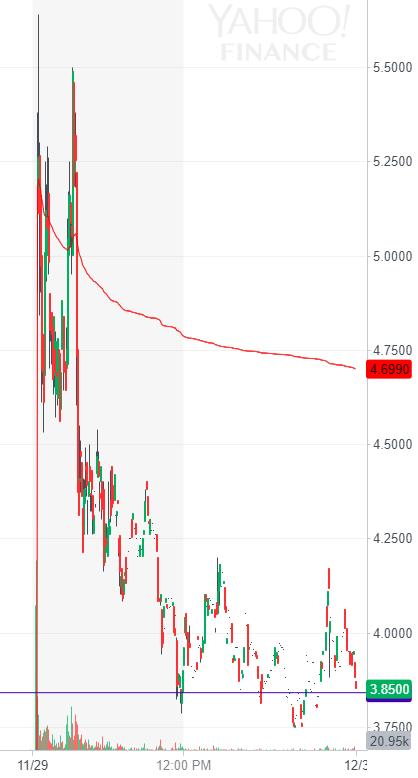
\includegraphics[width=200pt]{imgs/41.png}
    \caption{Day trading applications}
\end{figure}

\vspace{10pt}

\begin{figure}[!htb]
    \centering
    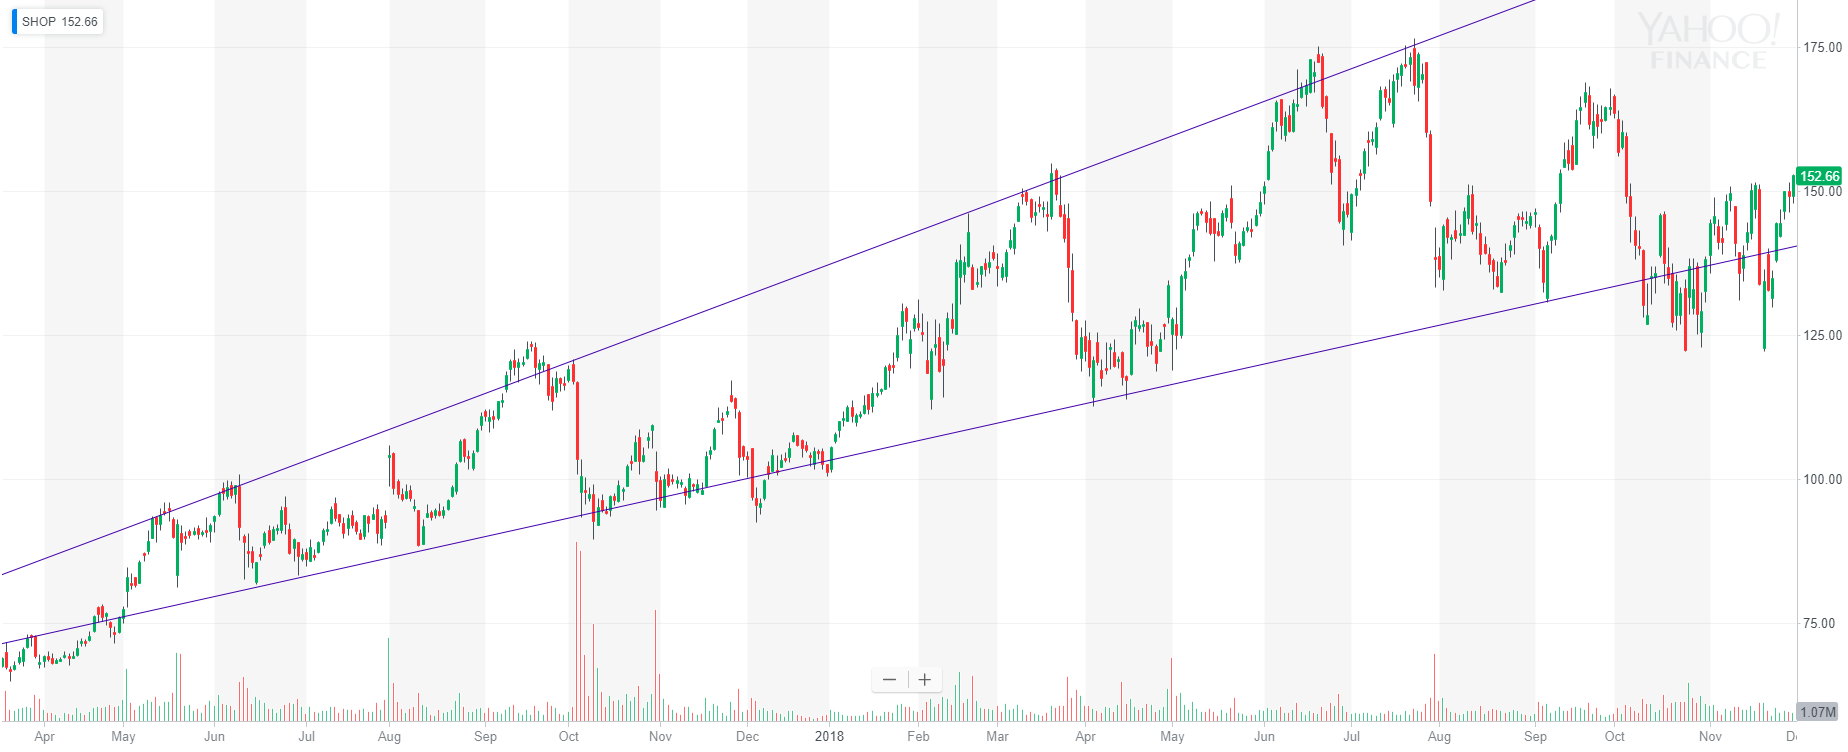
\includegraphics[width=\textwidth]{imgs/42.png}
    \caption{Linear support and resistance trends}
\end{figure}

\vspace{10pt}

\begin{figure}[!htb]
    \centering
    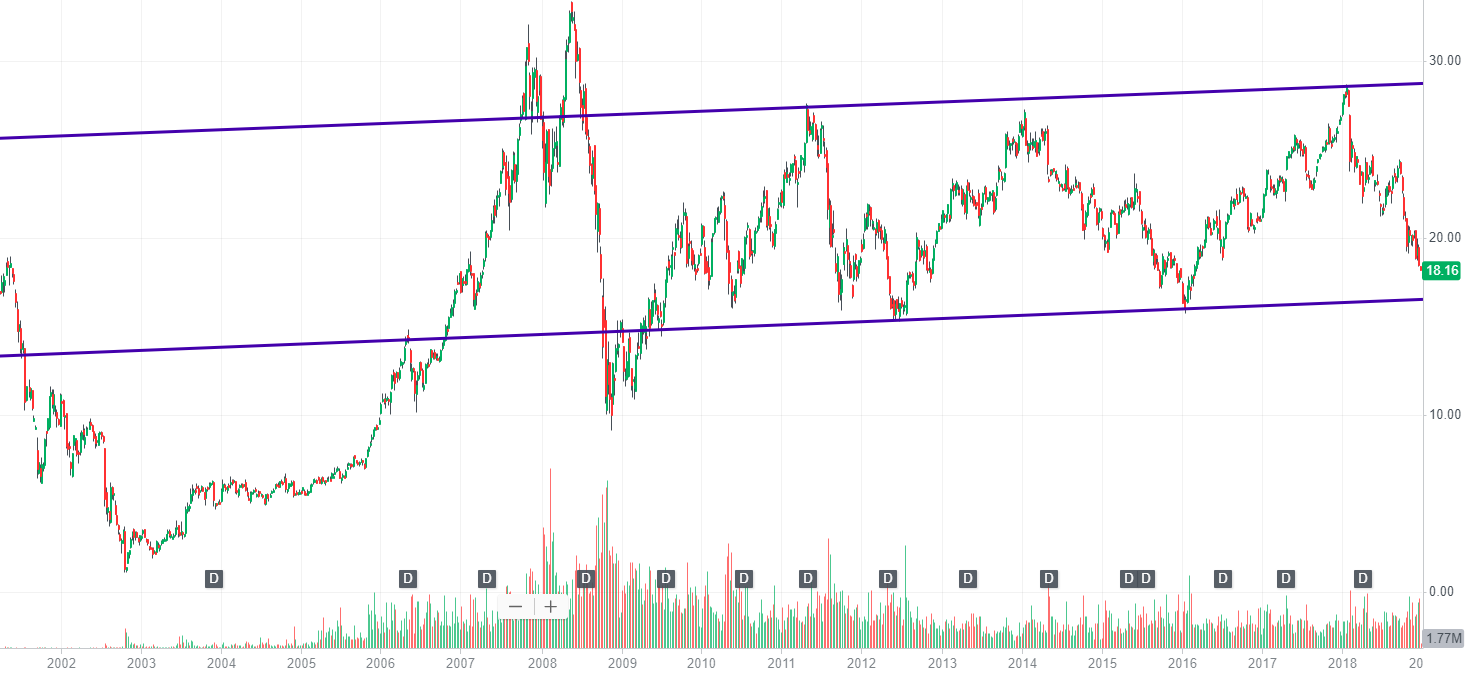
\includegraphics[width=\textwidth]{imgs/43.png}
    \caption{Forming an upward channel}
\end{figure}

\vspace{10pt}

\begin{figure}[!htb]
    \centering
    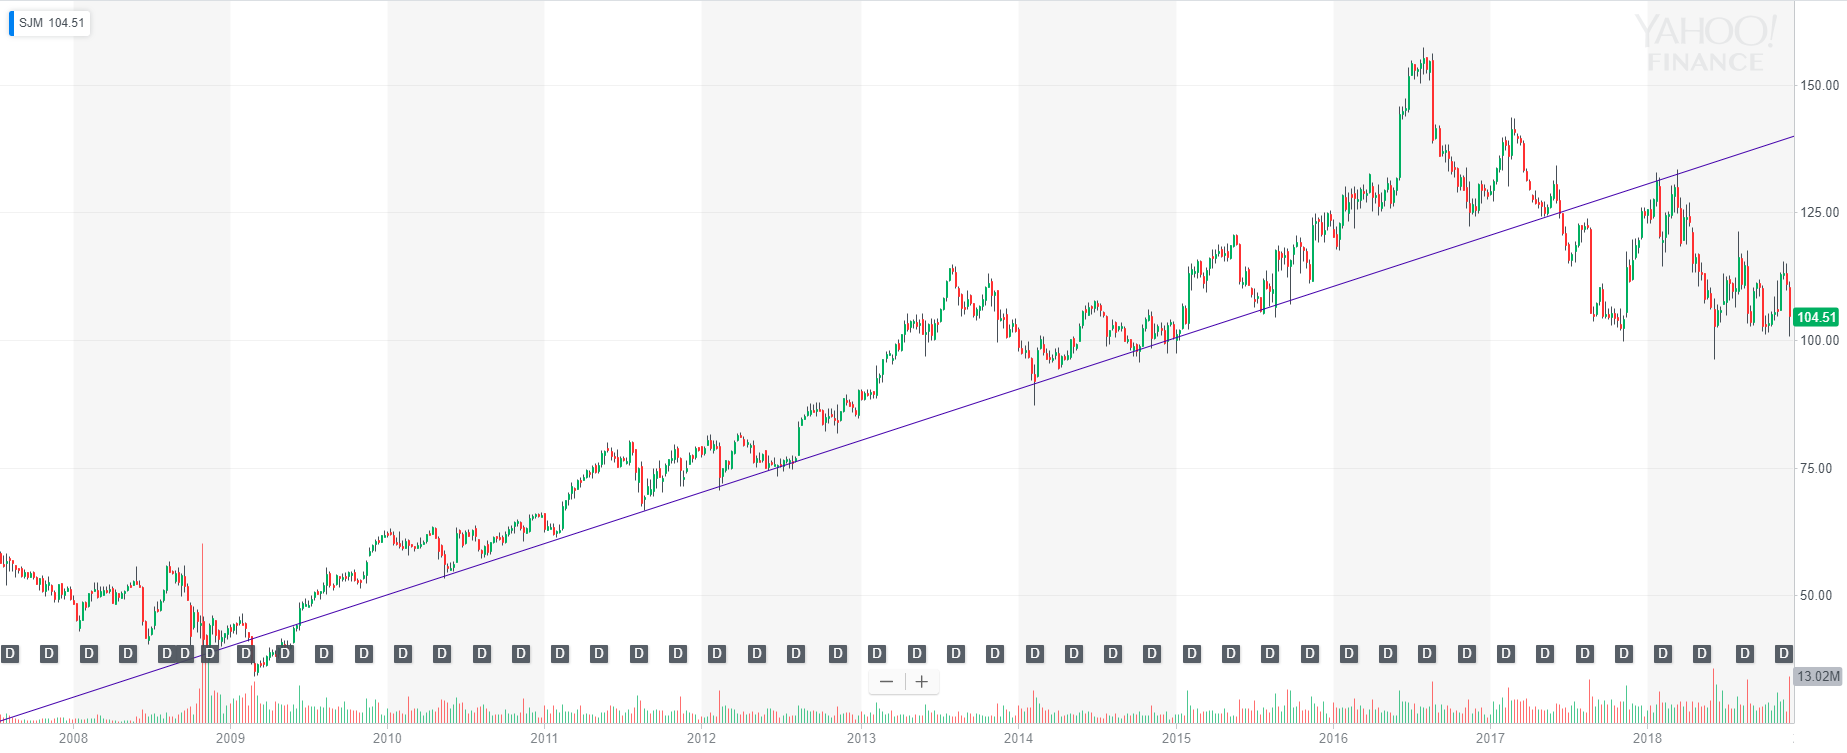
\includegraphics[width=\textwidth]{imgs/44.png}
    \caption{Unbounded linear support and breakout example}
\end{figure}

\vspace{10pt}

\begin{figure}[!htb]
    \centering
    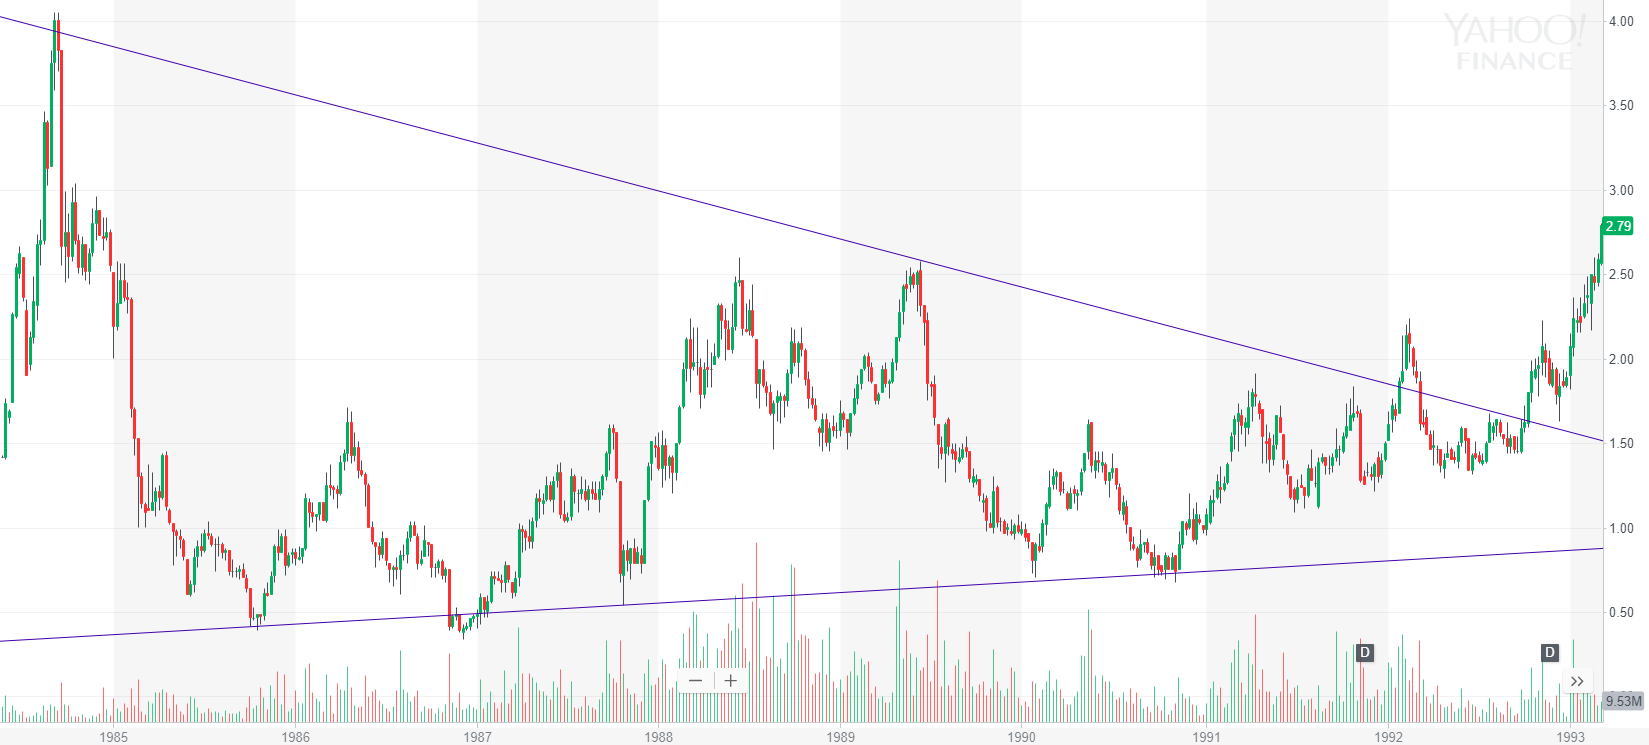
\includegraphics[width=\textwidth]{imgs/45.png}
    \caption{Introducing wedges}
\end{figure}

\vspace{10pt}

\begin{figure}[!htb]
    \centering
    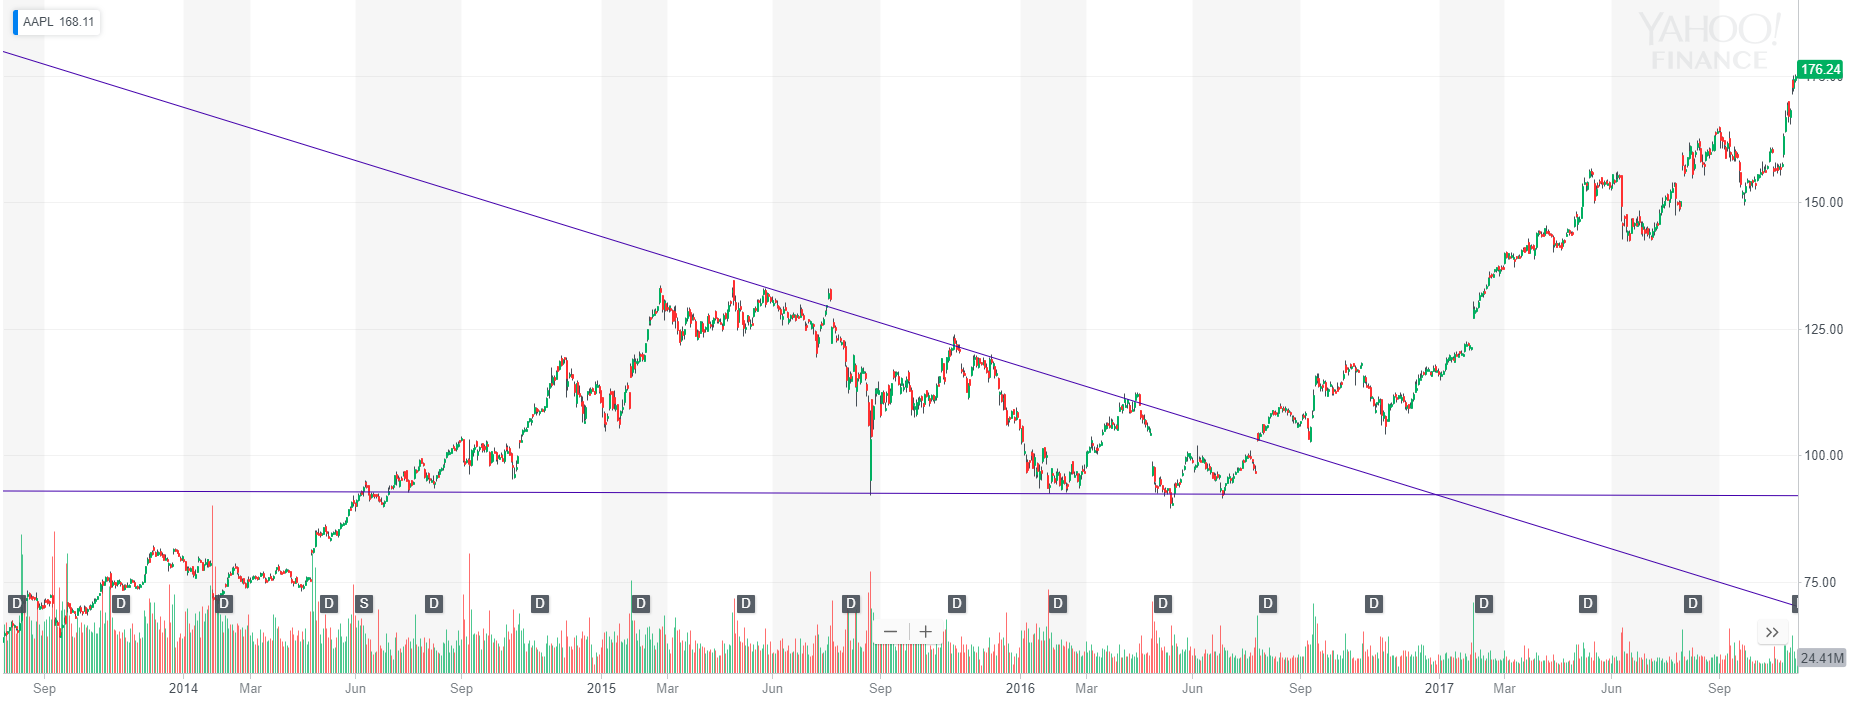
\includegraphics[width=\textwidth]{imgs/46.png}
    \caption{Downward wedges}
\end{figure}

\vspace{10pt}

\begin{figure}[!htb]
    \centering
    \includegraphics[width=\textwidth]{imgs/47.png}
    \caption{Upward wedges}
\end{figure}

\vspace{10pt}

\begin{figure}[!htb]
    \centering
    \includegraphics[width=\textwidth]{imgs/48.png}
    \caption{Volatility outside of precise support and resistance levels before a breakout}
\end{figure}

\vspace{10pt}

\begin{figure}[!htb]
    \centering
    \includegraphics[width=\textwidth]{imgs/49.png}
    \caption{Introducing price targets}
\end{figure}

\vspace{10pt}

\begin{figure}[!htb]
    \centering
    \includegraphics[width=\textwidth]{imgs/50.png}
    \caption{Wedge targets exemplified}
\end{figure}

\vspace{10pt}

\begin{figure}[!htb]
    \centering
    \includegraphics[width=500pt]{imgs/51.png}
    \caption{Trading and volatility implications}
\end{figure}

\vspace{10pt}

\begin{figure}[!htb]
    \centering
    \includegraphics[width=\textwidth]{imgs/52.png}
    \caption{Expected time to complete}
\end{figure}

\clearpage
\vspace*{.5in}

\begin{figure}[!htb]
    \centering
    \includegraphics[width=\textwidth]{imgs/53.png}
    \caption{Introducing flags}
\end{figure}

\begin{figure}[!htb]
    \centering
    \includegraphics[width=.5\textwidth]{imgs/54.png}
    \caption{Poles and potential continuation}
\end{figure}

\vspace{10pt}

\begin{figure}[!htb]
    \centering
    \includegraphics[width=.6\textwidth]{imgs/55.png}
    \caption{Setting precise targets}
\end{figure}

\vspace{10pt}

\begin{figure}[!htb]
    \centering
    \includegraphics[width=\textwidth]{imgs/56.png}
    \caption{Introducing the ABCD setup}
\end{figure}

\vspace{10pt}

\begin{figure}[!htb]
    \centering
    \includegraphics[width=\textwidth]{imgs/57.png}
    \caption{Identifying the B}
\end{figure}

\vspace{10pt}

\begin{figure}[!htb]
    \centering
    \includegraphics[width=\textwidth]{imgs/58.png}
    \caption{Waiting for consolidation}
\end{figure}

\vspace{10pt}

\begin{figure}[!htb]
    \centering
    \includegraphics[width=\textwidth]{imgs/59.png}
    \caption{Value recognition}
\end{figure}

\vspace{10pt}

\begin{figure}[!htb]
    \centering
    \includegraphics[width=\textwidth]{imgs/60.png}
    \caption{\href{https://ninetonoonsecrets.com/imgs/60.png}{The ABCD setup}}
\end{figure}

\vspace{10pt}

\begin{figure}[!htb]
    \centering
    \includegraphics[width=\textwidth]{imgs/61.png}
    \caption{The ABCD setup vs cup and handle}
\end{figure}

\vspace{10pt}

\begin{figure}[!htb]
    \centering
    \includegraphics[width=.7\textwidth]{imgs/62.png}
    \caption{Investopedia depiction}
\end{figure}

\vspace{10pt}

\begin{figure}[!htb]
    \centering
    \includegraphics[width=\textwidth]{imgs/63.png}
    \caption{Introducing the head and shoulders setup}
\end{figure}

\vspace{10pt}

\begin{figure}[!htb]
    \centering
    \includegraphics[width=\textwidth]{imgs/64.png}
    \caption{Identifying the shoulder-neckline price range}
\end{figure}

\vspace{10pt}

\begin{figure}[!htb]
    \centering
    \includegraphics[width=\textwidth]{imgs/65.png}
    \caption{Implications and setting targets}
\end{figure}

\vspace{10pt}

\begin{figure}[!htb]
    \centering
    \includegraphics[width=\textwidth]{imgs/66.png}
    \caption{Foundations for inverse pattern}
\end{figure}

\vspace{10pt}

\begin{figure}[!htb]
    \centering
    \includegraphics[width=\textwidth]{imgs/67.png}
    \caption{\href{https://ninetonoonsecrets.com/imgs/67.png}{Inverse head and shoulders setup}}
\end{figure}

\vspace{10pt}

\begin{figure}[!htb]
    \centering
    \includegraphics[width=.56\textwidth]{imgs/68.png}
    \caption{Introducing hammer candles}
\end{figure}

\vspace{10pt}

\begin{figure}[!htb]
    \centering
    \includegraphics[width=\textwidth]{imgs/69.png}
    \caption{Use in turnarounds}
\end{figure}

\vspace{10pt}

\begin{figure}[!htb]
    \centering
    \includegraphics[width=\textwidth]{imgs/70.png}
    \caption{Expanding candlestick patterns}
\end{figure}

\vspace{10pt}

\begin{figure}[!htb]
    \centering
    \includegraphics[width=\textwidth]{imgs/71.png}
    \caption{Inverted uses}
\end{figure}

\vspace{10pt}

\begin{figure}[!htb]
    \centering
    \includegraphics[width=\textwidth]{imgs/72.png}
    \caption{Introducing moving averages}
\end{figure}

\vspace{10pt}

\begin{figure}[!htb]
    \centering
    \includegraphics[width=\textwidth]{imgs/73.png}
    \caption{Mean reversion}
\end{figure}

\vspace{10pt}

\begin{figure}[!htb]
    \centering
    \includegraphics[width=\textwidth]{imgs/74.png}
    \caption{Setting targets with support levels}
\end{figure}

\vspace{10pt}

\begin{figure}[!htb]
    \centering
    \includegraphics[width=\textwidth]{imgs/75.png}
    \caption{Combining indicators for greater insights}
\end{figure}

\vspace{10pt}

\begin{figure}[!htb]
    \centering
    \includegraphics[width=\textwidth]{imgs/76.png}
    \caption{Identifying dominant indicator factors}
\end{figure}

\vspace{10pt}

\begin{figure}[!htb]
    \centering
    \includegraphics[width=\textwidth]{imgs/77.png}
    \caption{Impacts based on long-term trends}
\end{figure}

\vspace{10pt}

\begin{figure}[!htb]
    \centering
    \includegraphics[width=\textwidth]{imgs/78.png}
    \caption{Modifying math factors to extract tradable barometers}
\end{figure}

\vspace{10pt}

\begin{figure}[!htb]
    \centering
    \includegraphics[width=\textwidth]{imgs/79.png}
    \caption{Trendlines in indicators}
\end{figure}

\vspace{10pt}

\begin{figure}[!htb]
    \centering
    \includegraphics[width=\textwidth]{imgs/80.png}
    \caption{Turning indicator trends into swing trades}
\end{figure}

\vspace{10pt}

\begin{figure}[!htb]
    \centering
    \includegraphics[width=.5\textwidth]{imgs/81.png}
    \caption{Stochastics nuances}
\end{figure}

\vspace{10pt}

\begin{figure}[!htb]
    \centering
    \includegraphics[width=\textwidth]{imgs/82.png}
    \caption{Insights from market trends}
\end{figure}

\vspace{10pt}

\begin{figure}[!htb]
    \centering
    \includegraphics[width=\textwidth]{imgs/83.png}
    \caption{Understanding divergence}
\end{figure}

\vspace{10pt}

\begin{figure}[!htb]
    \centering
    \includegraphics[width=\textwidth]{imgs/84.png}
    \caption{Modifying parameters}
\end{figure}

\vspace{10pt}

\begin{figure}[!htb]
    \centering
    \includegraphics[width=\textwidth]{imgs/85.png}
    \caption{Introducing Bollinger Bands}
\end{figure}

\vspace{10pt}

\begin{figure}[!htb]
    \centering
    \includegraphics[width=\textwidth]{imgs/86.png}
    \caption{Quantifying volatility}
\end{figure}

\vspace{10pt}

\begin{figure}[!htb]
    \centering
    \includegraphics[width=.86\textwidth]{imgs/87.png}
    \caption{Introducing the interior Bollinger Band M setup}
\end{figure}

\vspace{10pt}

\begin{figure}[!htb]
    \centering
    \includegraphics[width=.86\textwidth]{imgs/88.png}
    \caption{Inverse interior Bollinger Band W setup}
\end{figure}

\vspace{10pt}

\begin{figure}[!htb]
    \centering
    \includegraphics[width=\textwidth]{imgs/89.png}
    \caption{Individual Bollinger characteristics and implications}
\end{figure}

\vspace{10pt}

\begin{figure}[!htb]
    \centering
    \includegraphics[width=\textwidth]{imgs/90.png}
    \caption{Introducing VWAP}
\end{figure}

\vspace{10pt}

\begin{figure}[!htb]
    \centering
    \includegraphics[width=\textwidth]{imgs/91.png}
    \caption{VWAP significance}
\end{figure}

\vspace{10pt}

\begin{figure}[!htb]
    \centering
    \includegraphics[width=\textwidth]{imgs/92.png}
    \caption{VWAP bands}
\end{figure}

\vspace{10pt}

\begin{figure}[!htb]
    \centering
    \includegraphics[width=\textwidth]{imgs/93.png}
    \caption{Circuit breakers}
\end{figure}

\vspace{10pt}

\begin{figure}[!htb]
    \centering
    \includegraphics[width=\textwidth]{imgs/94.png}
    \caption{Comprehensive analysis}
\end{figure}

\vspace{10pt}

\begin{figure}[!htb]
    \centering
    \includegraphics[width=\textwidth]{imgs/95.png}
    \caption{Nuanced analysis based on learned skills}
\end{figure}

\vspace{10pt}

\begin{figure}[!htb]
    \centering
    \includegraphics[width=\textwidth]{imgs/96.png}
    \caption{Identifying incredible breakouts with precise targets}
\end{figure}

\vspace{10pt}

\begin{figure}[!htb]
    \centering
    \includegraphics[width=.7\textwidth]{imgs/97.png}
    \caption{Introducing diversification}
\end{figure}

\clearpage
\vspace*{1in}

\begin{figure}[!htb]
    \centering
    \includegraphics[width=\textwidth]{imgs/98.png}
    \caption{Correlation exemplified through intra-industry comparisons}
\end{figure}

\vspace{10pt}

\begin{figure}[!htb]
    \centering
    \includegraphics[width=\textwidth]{imgs/99.png}
    \caption{Sector trend averages over time}
\end{figure}

\vspace{10pt}

\begin{figure}[!htb]
    \centering
    \includegraphics[width=\textwidth]{imgs/100.png}
    \caption{Portfolio structure}
\end{figure}

\vspace{10pt}

\begin{figure}[!htb]
    \centering
    \includegraphics[width=\textwidth]{imgs/101.png}
    \caption{Target funds for savings goals}
\end{figure}

\vspace{10pt}

\begin{figure}[!htb]
    \centering
    \includegraphics[width=\textwidth]{imgs/102.png}
    \caption{Eliminating risk with time}
\end{figure}

\vspace{10pt}

\begin{figure}[!htb]
    \centering
    \includegraphics[width=.9\textwidth]{imgs/103.png}
    \caption{\href{https://youtu.be/Nu4lHaSh7D4}{Ray Dalio's Holy Grail}}
\end{figure}

\vspace{10pt}

\begin{figure}[!htb]
    \centering
    \includegraphics[width=\textwidth]{imgs/104.png}
    \caption{General industry correlations}
\end{figure}

\vspace{10pt}

\begin{figure}[!htb]
    \centering
    \includegraphics[width=\textwidth]{imgs/105.png}
    \caption{International economic trends}
\end{figure}

\vspace{10pt}

\begin{figure}[!htb]
    \centering
    \includegraphics[width=.56\textwidth]{imgs/106.png}
    \caption{Implications related to correlation}
\end{figure}

\vspace{10pt}

\begin{figure}[!htb]
    \centering
    \includegraphics[width=\textwidth]{imgs/107.png}
    \caption{Example comparison of American and European markets}
\end{figure}

\vspace{10pt}

\begin{figure}[!htb]
    \centering
    \includegraphics[width=\textwidth]{imgs/108.png}
    \caption{Portfolio allocation examples}
\end{figure}

\vspace{10pt}

\begin{figure}[!htb]
    \centering
    \includegraphics[width=\textwidth]{imgs/109.png}
    \caption{Growth implications}
\end{figure}

\vspace{10pt}

\begin{figure}[!htb]
    \centering
    \includegraphics[width=\textwidth]{imgs/110.png}
    \caption{Ross Cameron's Profit Trifecta}
\end{figure}

\vspace{10pt}

\begin{figure}[!htb]
    \centering
    \includegraphics[width=\textwidth]{imgs/111.png}
    \caption{Implications of losing money}
\end{figure}

\vspace{10pt}

\begin{figure}[!htb]
    \centering
    \includegraphics[width=\textwidth]{imgs/112.png}
    \caption{Impact of position sizing}
\end{figure}

\vspace{10pt}

\begin{figure}[!htb]
    \centering
    \includegraphics[width=\textwidth]{imgs/113.png}
    \caption{Introducing premarket gainers}
\end{figure}

\vspace{10pt}

\begin{figure}[!htb]
    \centering
    \includegraphics[width=\textwidth]{imgs/114.png}
    \caption{Unique opportunities from open to noon}
\end{figure}

\vspace{10pt}

\begin{figure}[!htb]
    \centering
    \includegraphics[width=\textwidth]{imgs/115.png}
    \caption{Noon to close, and indicator implications}
\end{figure}

\vspace{10pt}

\begin{figure}[!htb]
    \centering
    \includegraphics[width=.5\textwidth]{imgs/116.png}
    \caption{Huge buy order with reporting delayed half an hour}
\end{figure}

\vspace{10pt}

\begin{figure}[!htb]
    \centering
    \includegraphics[width=.7\textwidth]{imgs/117.png}
    \caption{Something's wrong - Wall Street corrupted our system}
\end{figure}

\end{document}
